In this section, we compare results for the surging airfoil case based on meshes obtained from different adaptive strategies mentioned above. 
We compare different quantities of interest. 
A comparison of force response in the form of normalized lift and drag forces is shown in Figures \ref{fig:lift_plot} and \ref{fig:drag_plot} respectively. The normalized lift matches up well for all the meshes considered. Normalized drag shows differences only for Mz\_a2 mesh (the finest mesh), specifically between phases $\psi=160^\circ$ and $\psi=240^\circ$ whereas the drag response for all the other meshes matches up well.

A comparison of spanwise vorticity for the different meshes is shown in Figures \ref{fig:vorticity_195}, \ref{fig:vorticity_210}, and \ref{fig:vorticity_270} for phases $\psi=210^\circ$, $\psi=225^\circ$, and $\psi=270^\circ$, respectively.
For $\psi=195^\circ$, as the airfoil is in the retreating phase, boundary layer roll-up towards the geometric leading edge is observed over the airfoil surface. For the meshes based on zonal refinement, as we go from M0 to Mz\_a1 and Mz\_a2, the separation over the airfoil is well resolved, and more structures are visible as the mesh becomes finer. Comparing Mz\_a1, Ms\_a1, and Mf\_a1 meshes, we can see that Ms\_a1 mesh does not capture the fine-scale flow structures as compared to the Mz\_a1 mesh, both over the airfoil surface and in the wake of the airfoil. On the other hand, the Mf\_a1 mesh captures these fine-scale flow structures.

\begin{figure}[H]
\centering

\begin{subfigure}[b]{0.7\textwidth}
\centering
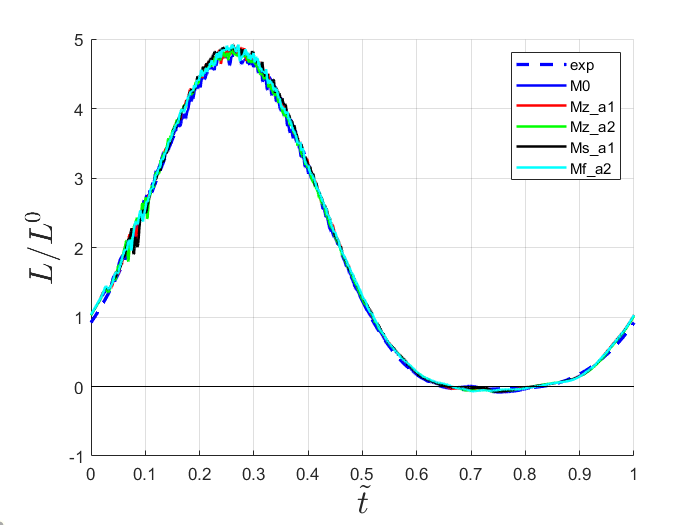
\includegraphics[width=1\textwidth]{figures/Results/Lift_plot.png}
\caption{Normalized lift}
\label{fig:lift_plot}
\end{subfigure}
\begin{subfigure}[b]{0.7\textwidth}
\centering
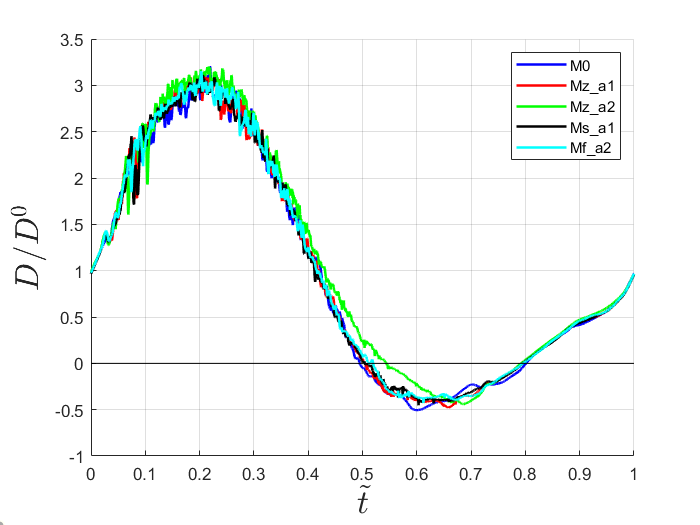
\includegraphics[width=1\textwidth]{figures/Results/Drag_plot.png}
\caption{Normalized drag}
\label{fig:drag_plot}
\end{subfigure}

\label{fig:force_response_adapt}
\caption{Normalized forces for different meshes}
\end{figure}

%Next, we look at the location of the LEV core for different meshes in Figure \ref{fig:LEV_location}. Some differences in the LEV location for various phases are observed. LEV location for Ma1, FB, and hadapt meshes is similar in the beginning phases. Ma1 starts to deviate from FB and hadapt in the later phases. LEV location for FB and hadapt meshes start to match with Ma2 in the later phases, whereas M0 LEV location fluctuates around the other meshes. This however is still not conclusive as to which mesh performs better and a more quantitative study is needed.


%%\begin{figure}[H]
%\centering
%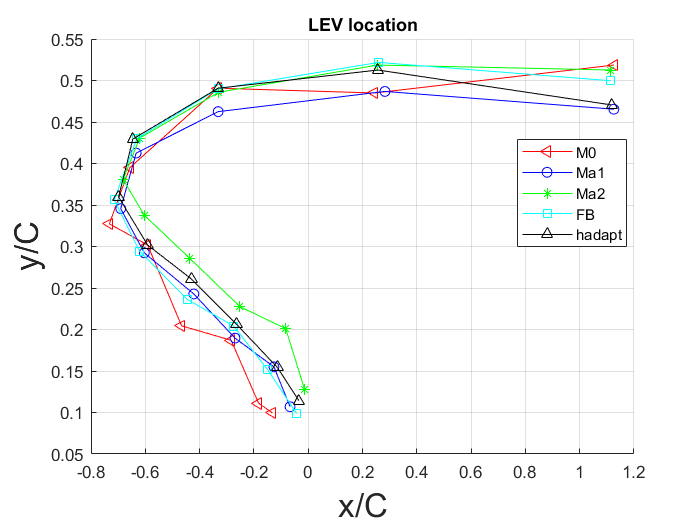
\includegraphics[width=0.7\textwidth]{figures/Results/LEV_location.png}
%\caption{LEV location for different meshes}
%\label{fig:LEV_location}
%\end{figure}
%%


For $\psi=210^\circ$, formation of LEV begins to take place, as we see a distinct vortex build up near the geometric leading edge. At this phase, the differences in the structures resolved by the different meshes become more clear, with Mz\_a2 being the most resolved. Similar to $\psi=195$, the Ms\_a1 mesh shows poor resolution of the fine-scale flow structures as compared to  Mz\_a1 and Mf\_a1 meshes.

For $\psi=270^\circ$, differences can be seen in the shear layer at the geometric leading edge of the airfoil, and the resolution of the LEV. The LEV and the shear layer are best resolved for Mz\_a2 and Mf\_a1 meshes. Recall that Mf\_a1 is obtained using feature-based mesh refinement designed to resolve the LEV accurately, and has the same mesh resolution as Mz\_a2 along the path of the LEV. Once again, shear layer is not well resolved for Ms\_a1 as compared to other refined/adapted meshes.

The poor resolution of the flow-field observed for Ms\_a1 can be attributed to the mesh not having a uniform refinement in the regions of interest, having been adapted solely based on the error-field obtained, which results in a patchy mesh, i.e., the mesh size does not remain constant in particular zones, and hence, structures are not resolved as desired.

\begin{figure}[H]
\centering
\begin{subfigure}[b]{0.475\textwidth}
\centering
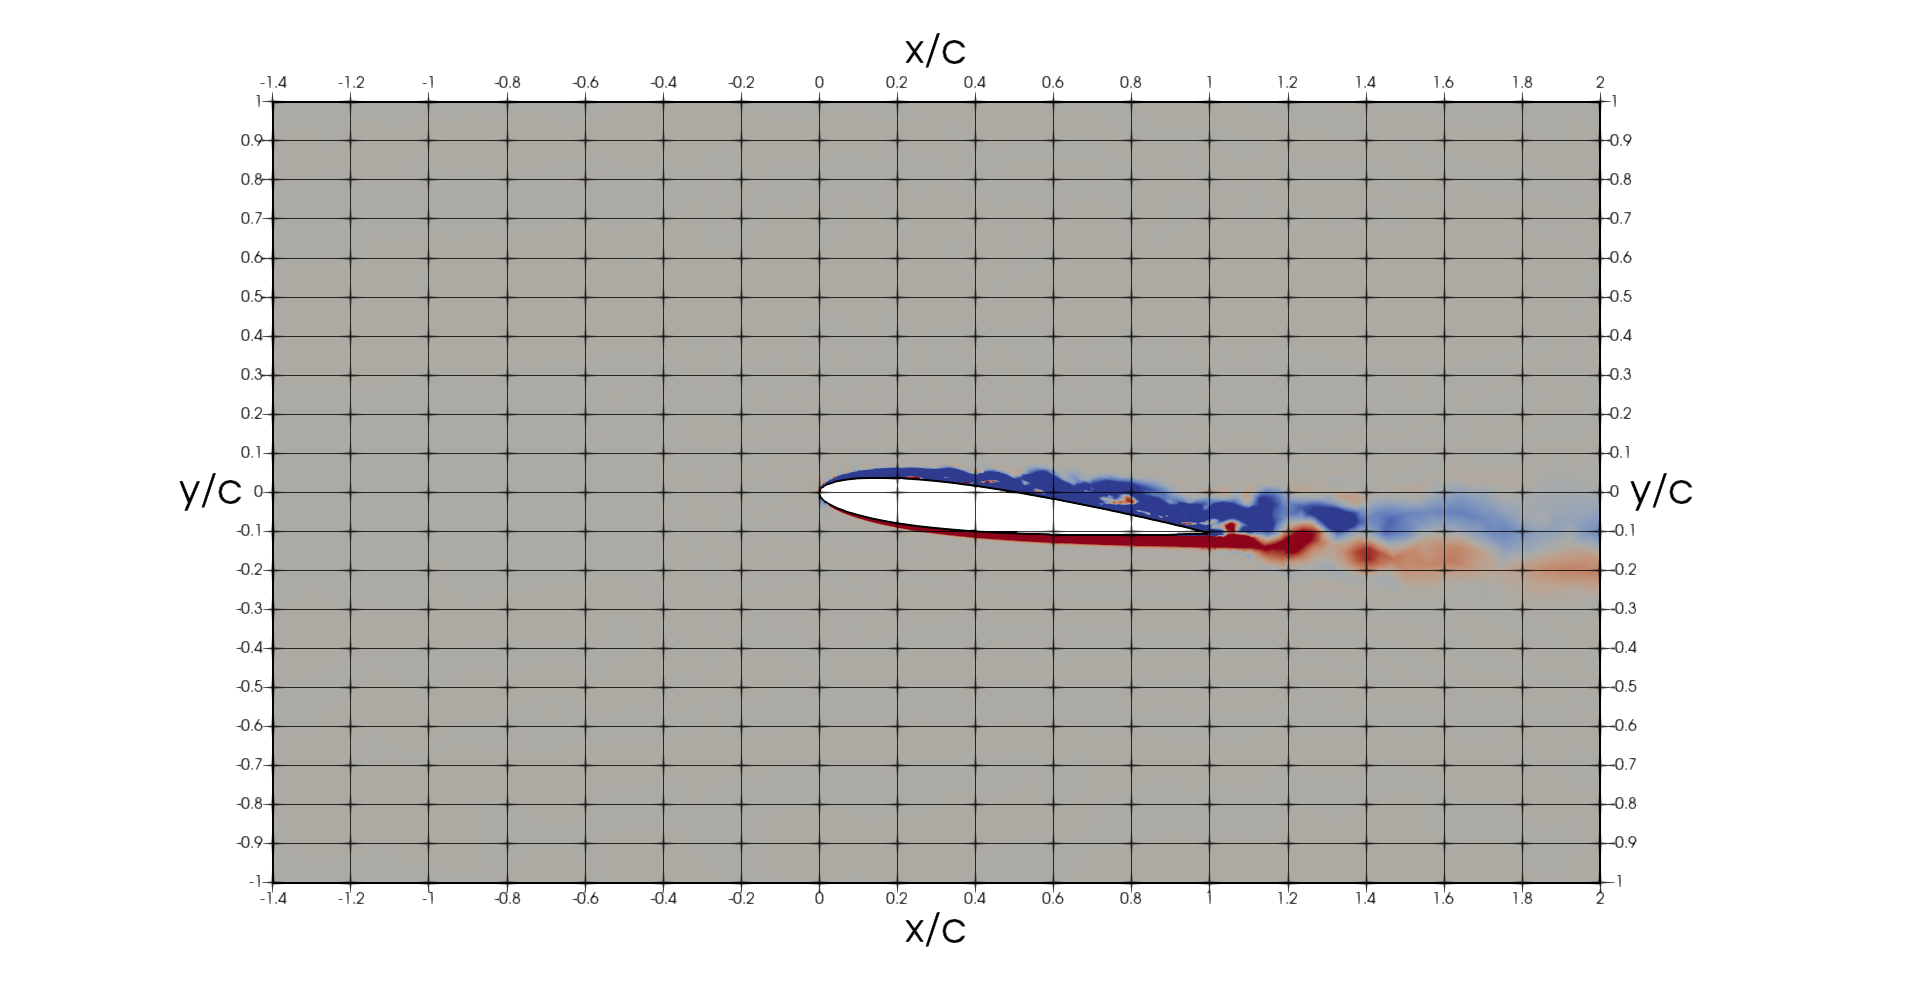
\includegraphics[width=1.25\textwidth]{figures/vorticity_plots/M0/ph_195.png}
\caption{M0 mesh, $\psi$ = $195^\circ$}
\label{fig:M0_psi195}
\end{subfigure}
\begin{subfigure}[b]{0.475\textwidth}
\centering
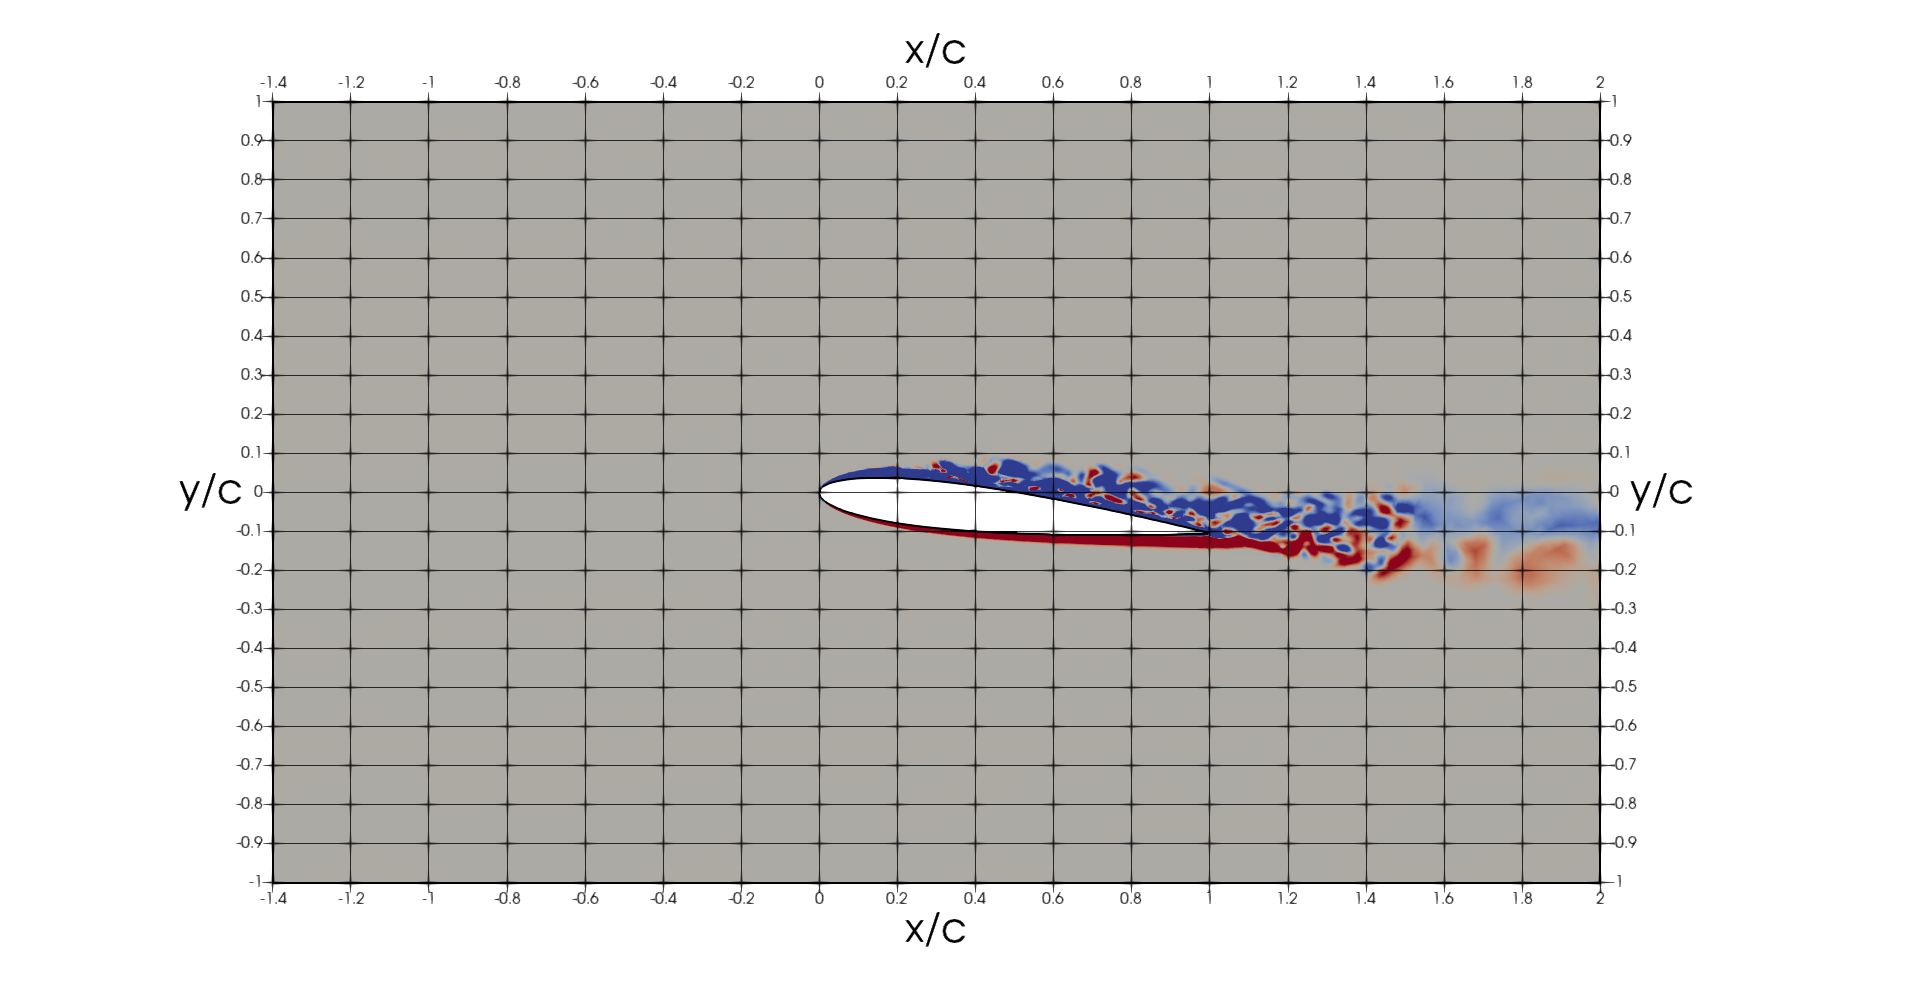
\includegraphics[width=1.25\textwidth]{figures/vorticity_plots/Mza1/ph_195.png}
\caption{Mz\_a1 mesh, $\psi$ = $195^\circ$}
\label{fig:Ma1_psi195}
\end{subfigure}
\begin{subfigure}[b]{0.475\textwidth}
\centering
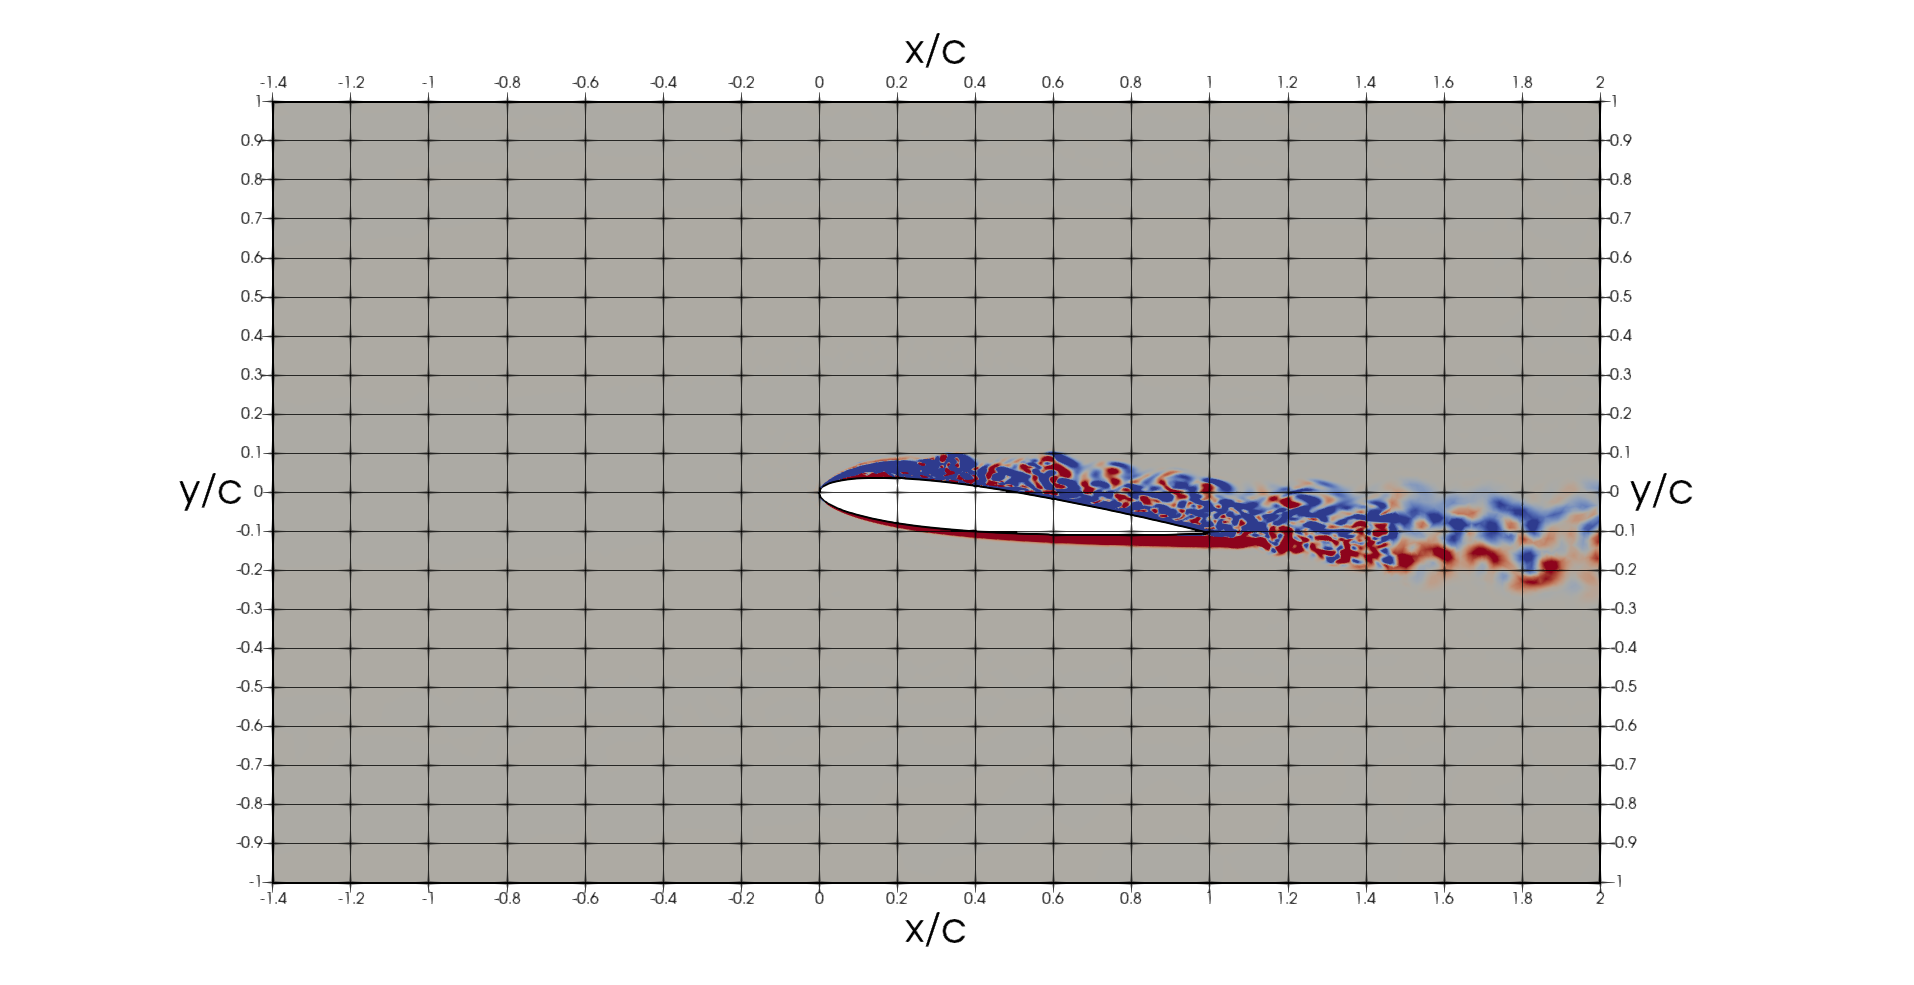
\includegraphics[width=1.25\textwidth]{figures/vorticity_plots/Mza2/ph_195.png}
\caption{Mz\_a2 mesh, $\psi$ = $195^\circ$}
\label{fig:Ma2_psi195}
\end{subfigure}
\begin{subfigure}[b]{0.475\textwidth}
\centering
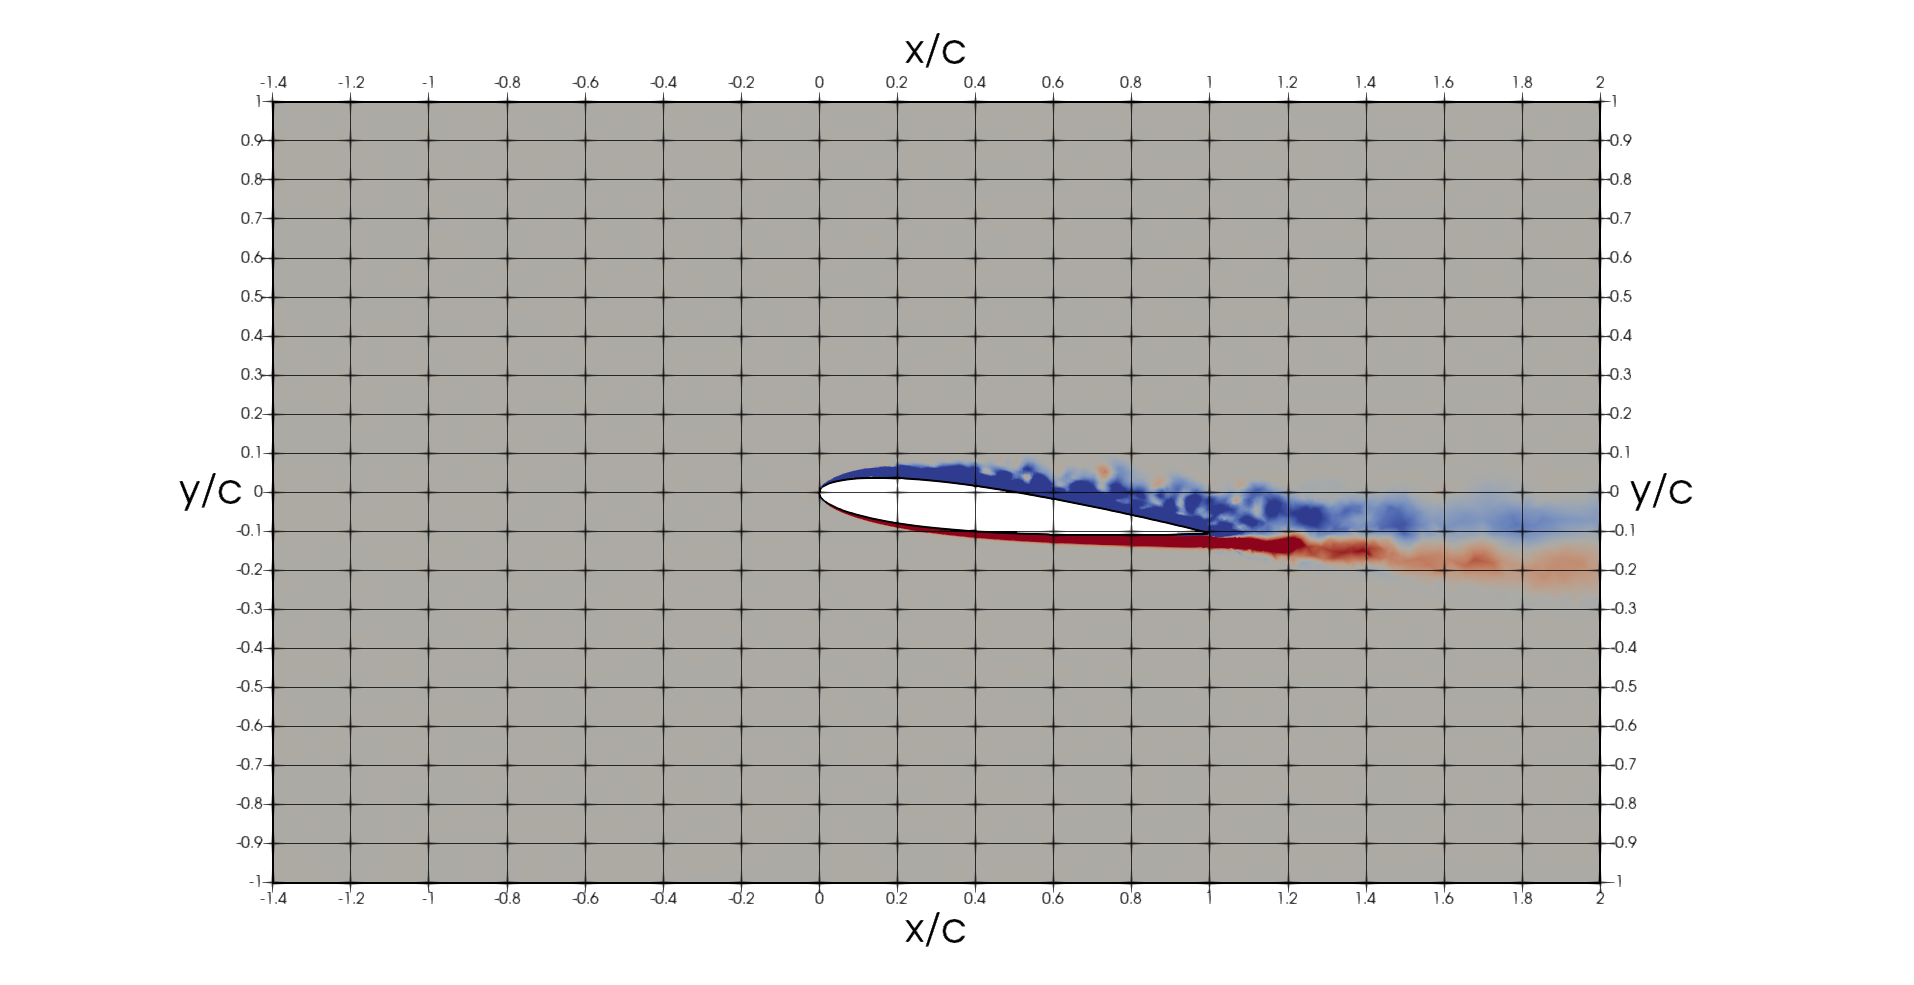
\includegraphics[width=1.25\textwidth]{figures/vorticity_plots/SB/ph_195.png}
\caption{Ms\_a1 mesh, $\psi$ = $195^\circ$}
\label{fig:hadapt_psi195}
\end{subfigure}

\begin{subfigure}[b]{0.475\textwidth}
\centering
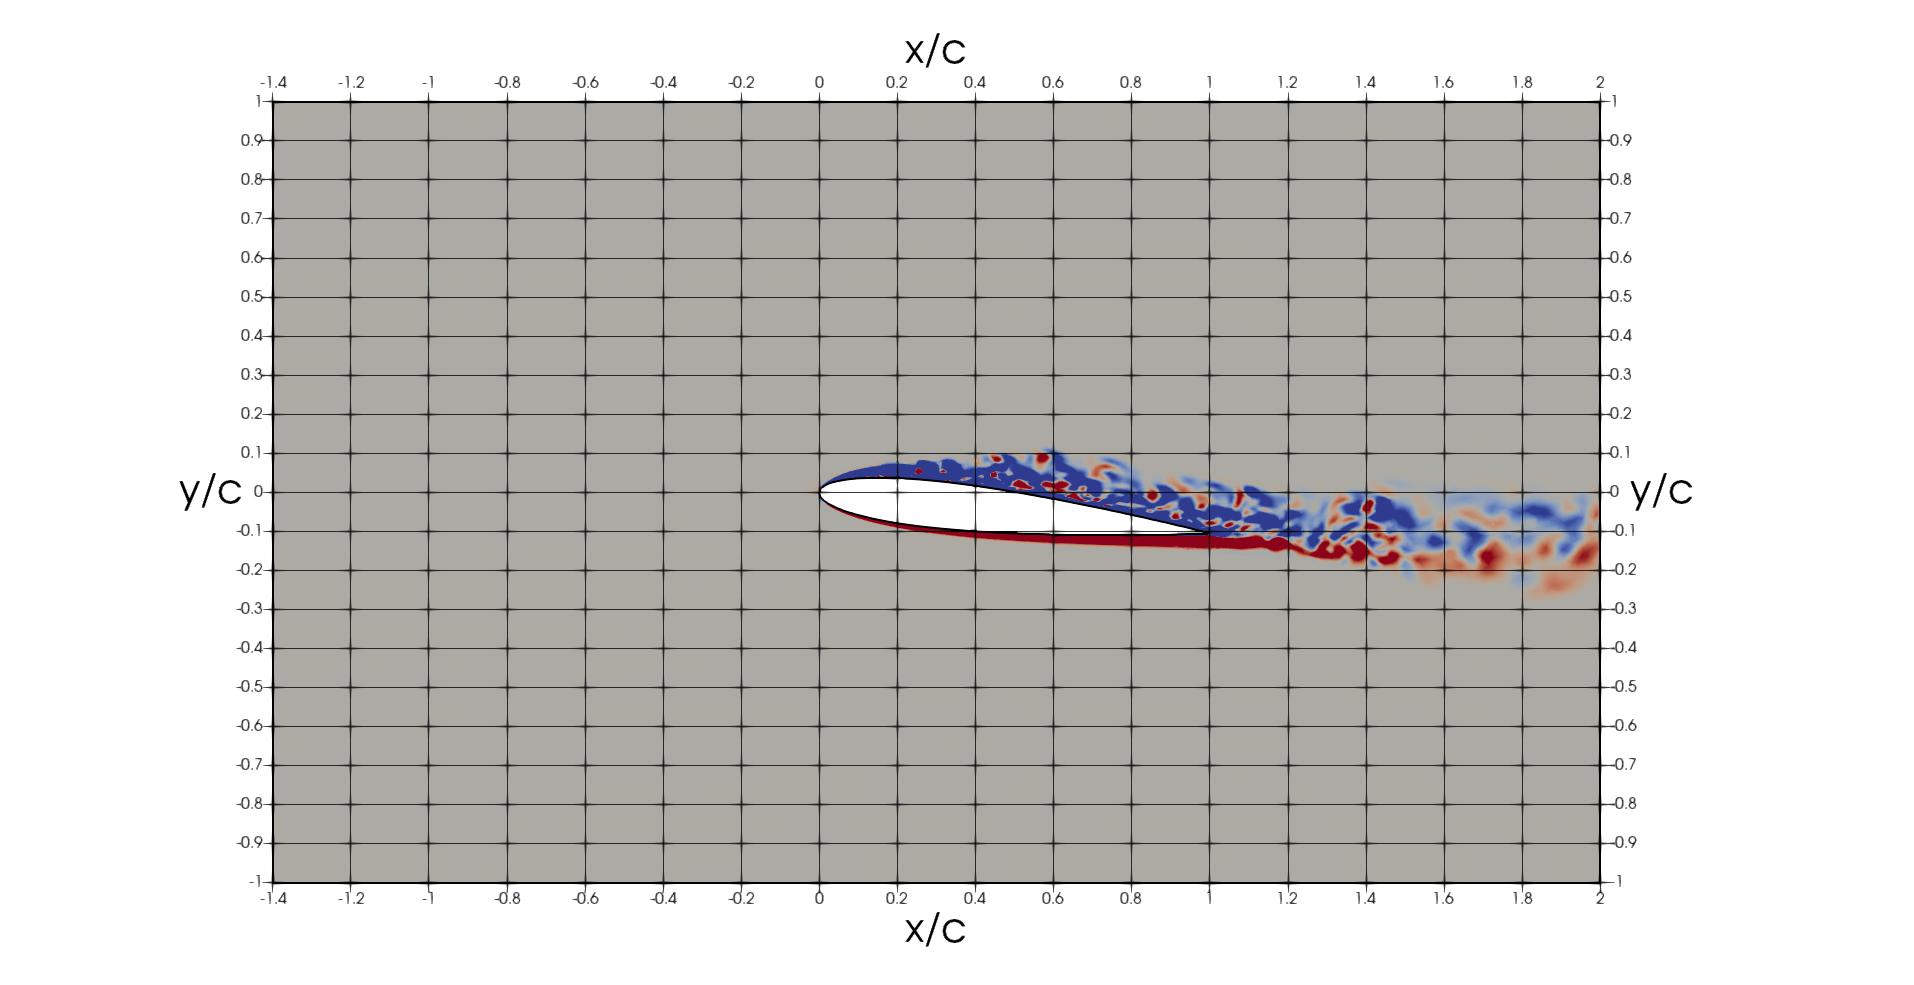
\includegraphics[width=1.25\textwidth]{figures/vorticity_plots/FB/ph_195.png}
\caption{Mf\_a1 mesh, $\psi$ = $195^\circ$}
\label{fig:FB_psi195}
\end{subfigure}
\caption{Spanwise vorticity comparison at $\psi$ = $195^\circ$ for different meshes}
\label{fig:vorticity_195}
\end{figure}



\begin{figure}[H]
\centering
\begin{subfigure}[b]{0.475\textwidth}
\centering
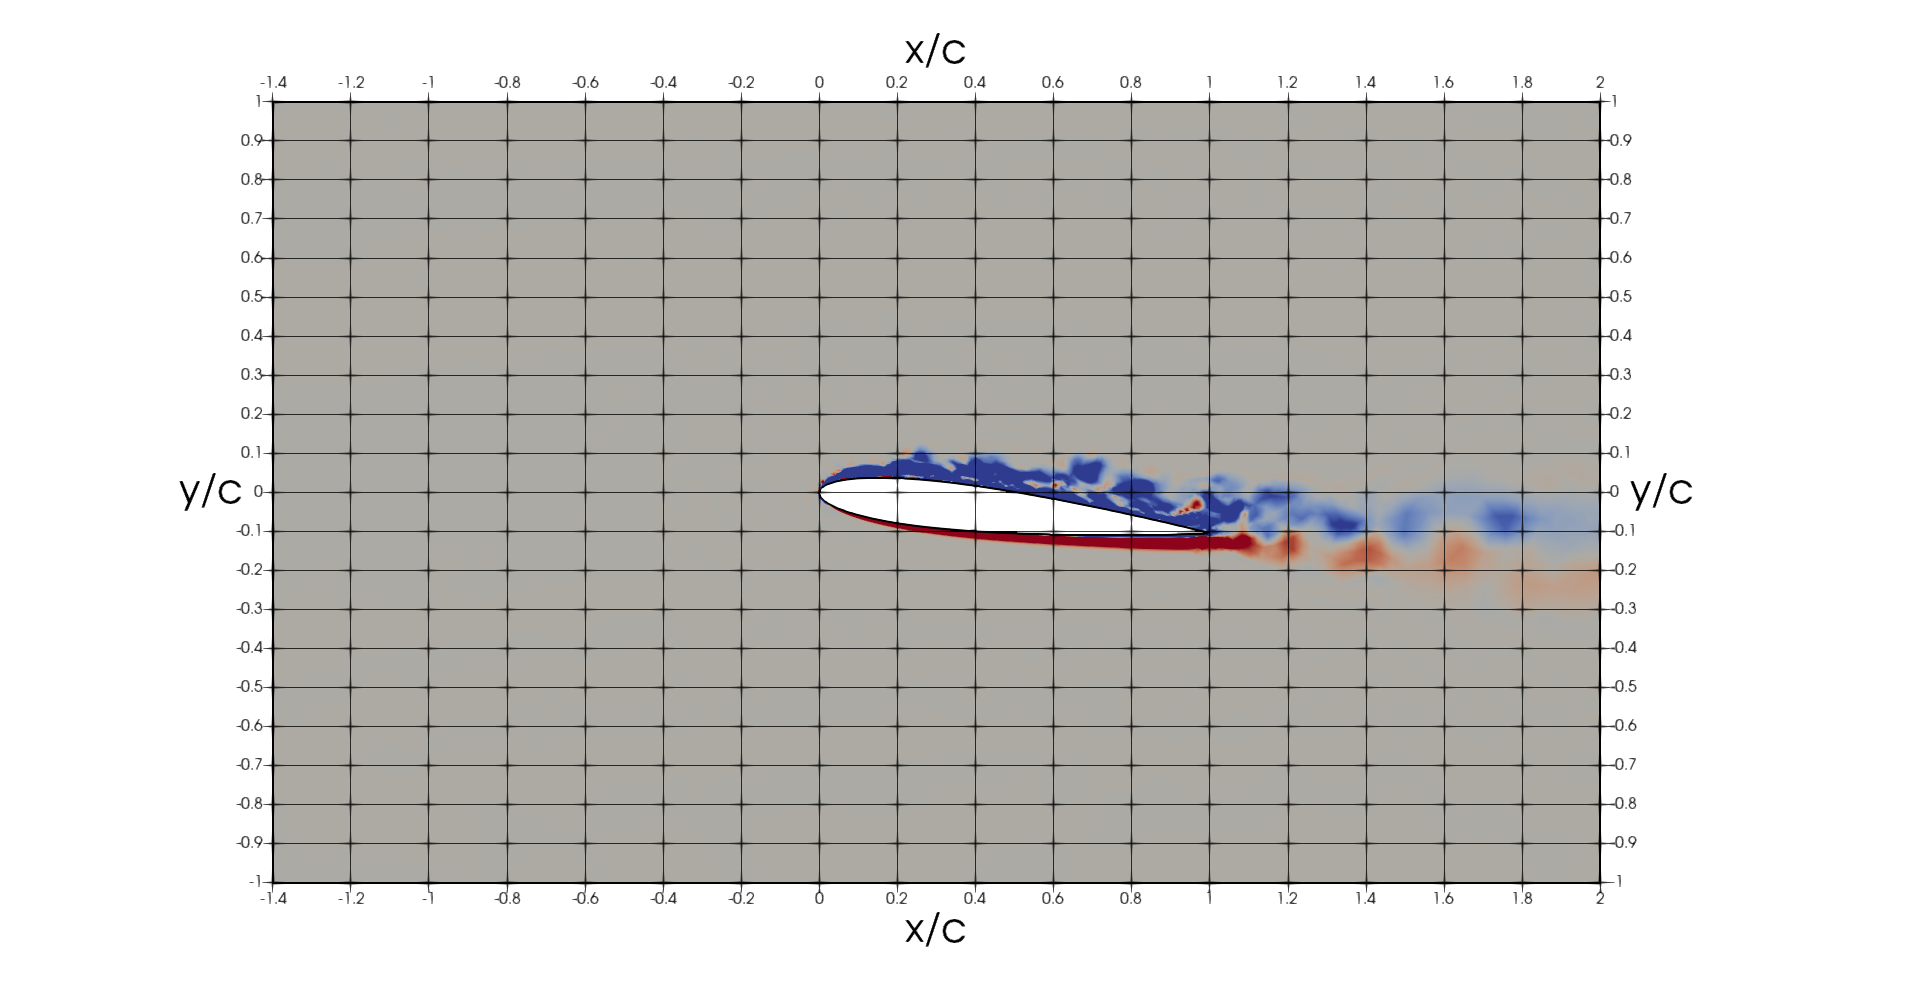
\includegraphics[width=1.25\textwidth]{figures/vorticity_plots/M0/ph_210.png}
\caption{M0 mesh, $\psi$ = $210^\circ$}
\label{fig:M0_psi210}
\end{subfigure}
\begin{subfigure}[b]{0.475\textwidth}
\centering
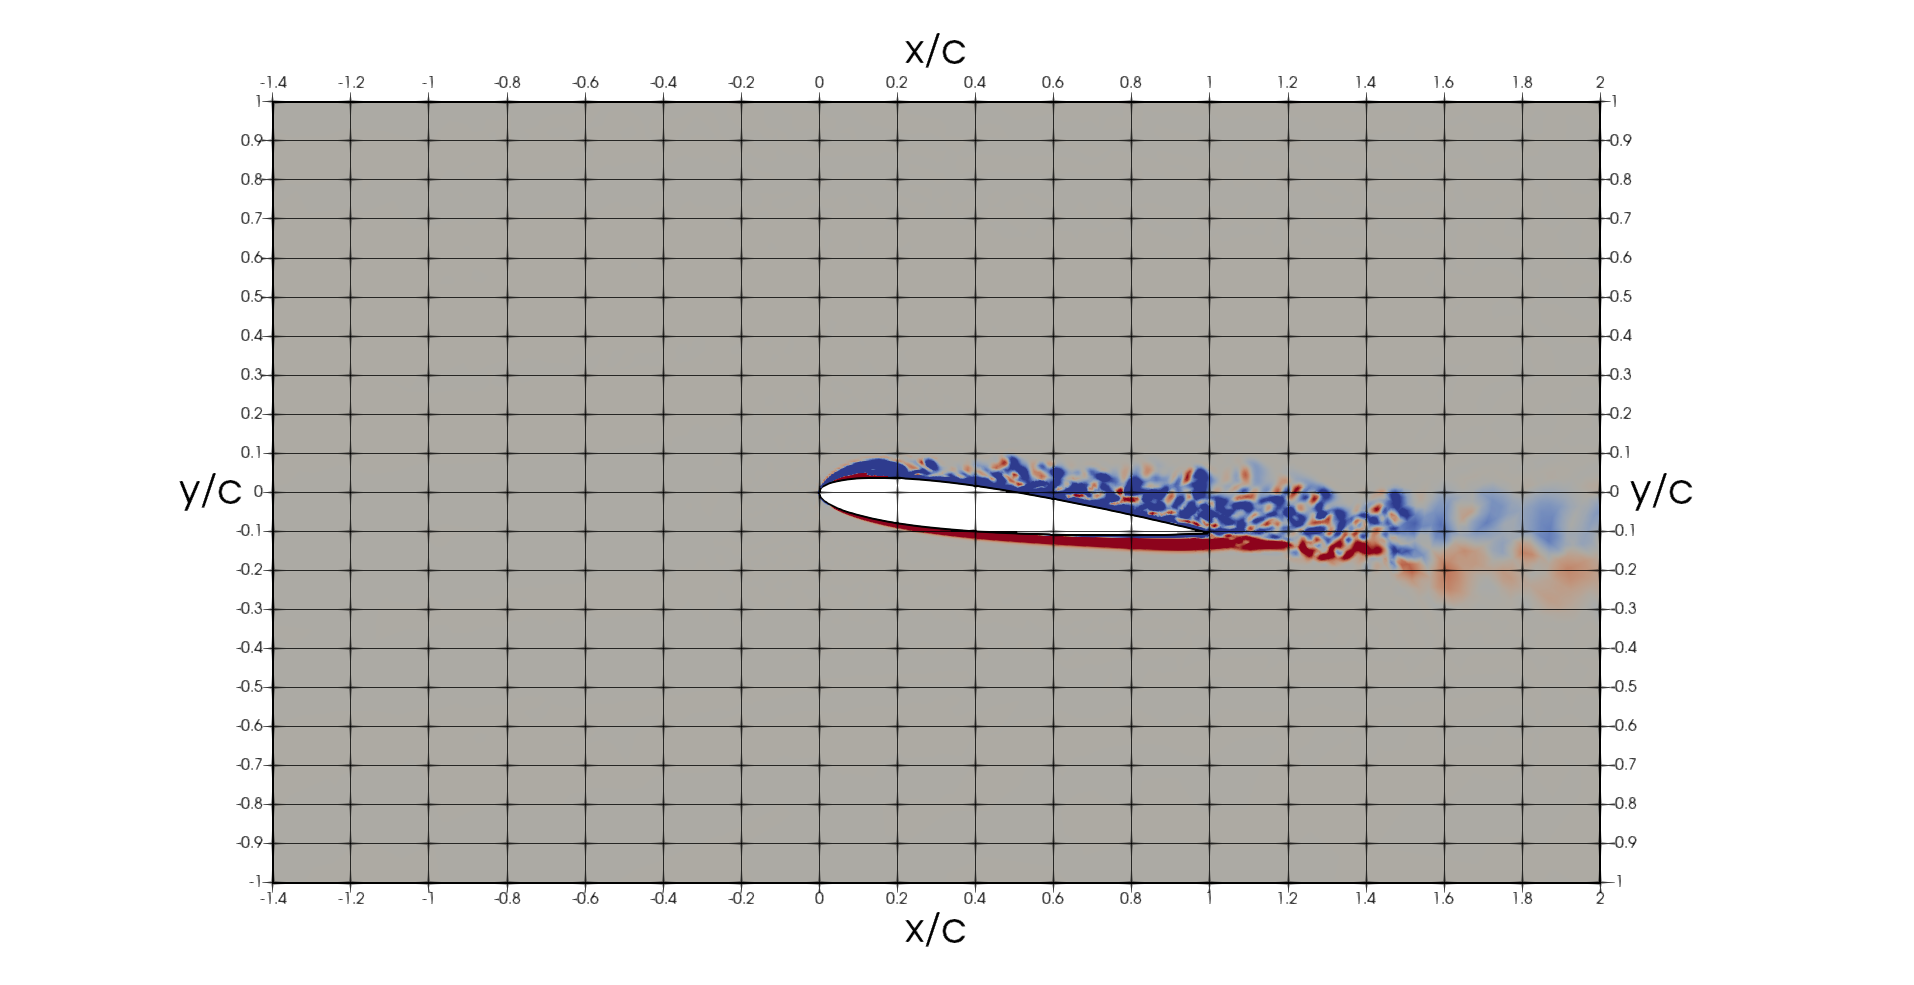
\includegraphics[width=1.25\textwidth]{figures/vorticity_plots/Mza1/ph_210.png}
\caption{Mz\_a1 mesh, $\psi$ = $210^\circ$}
\label{fig:Ma1_psi210}
\end{subfigure}
\begin{subfigure}[b]{0.475\textwidth}
\centering
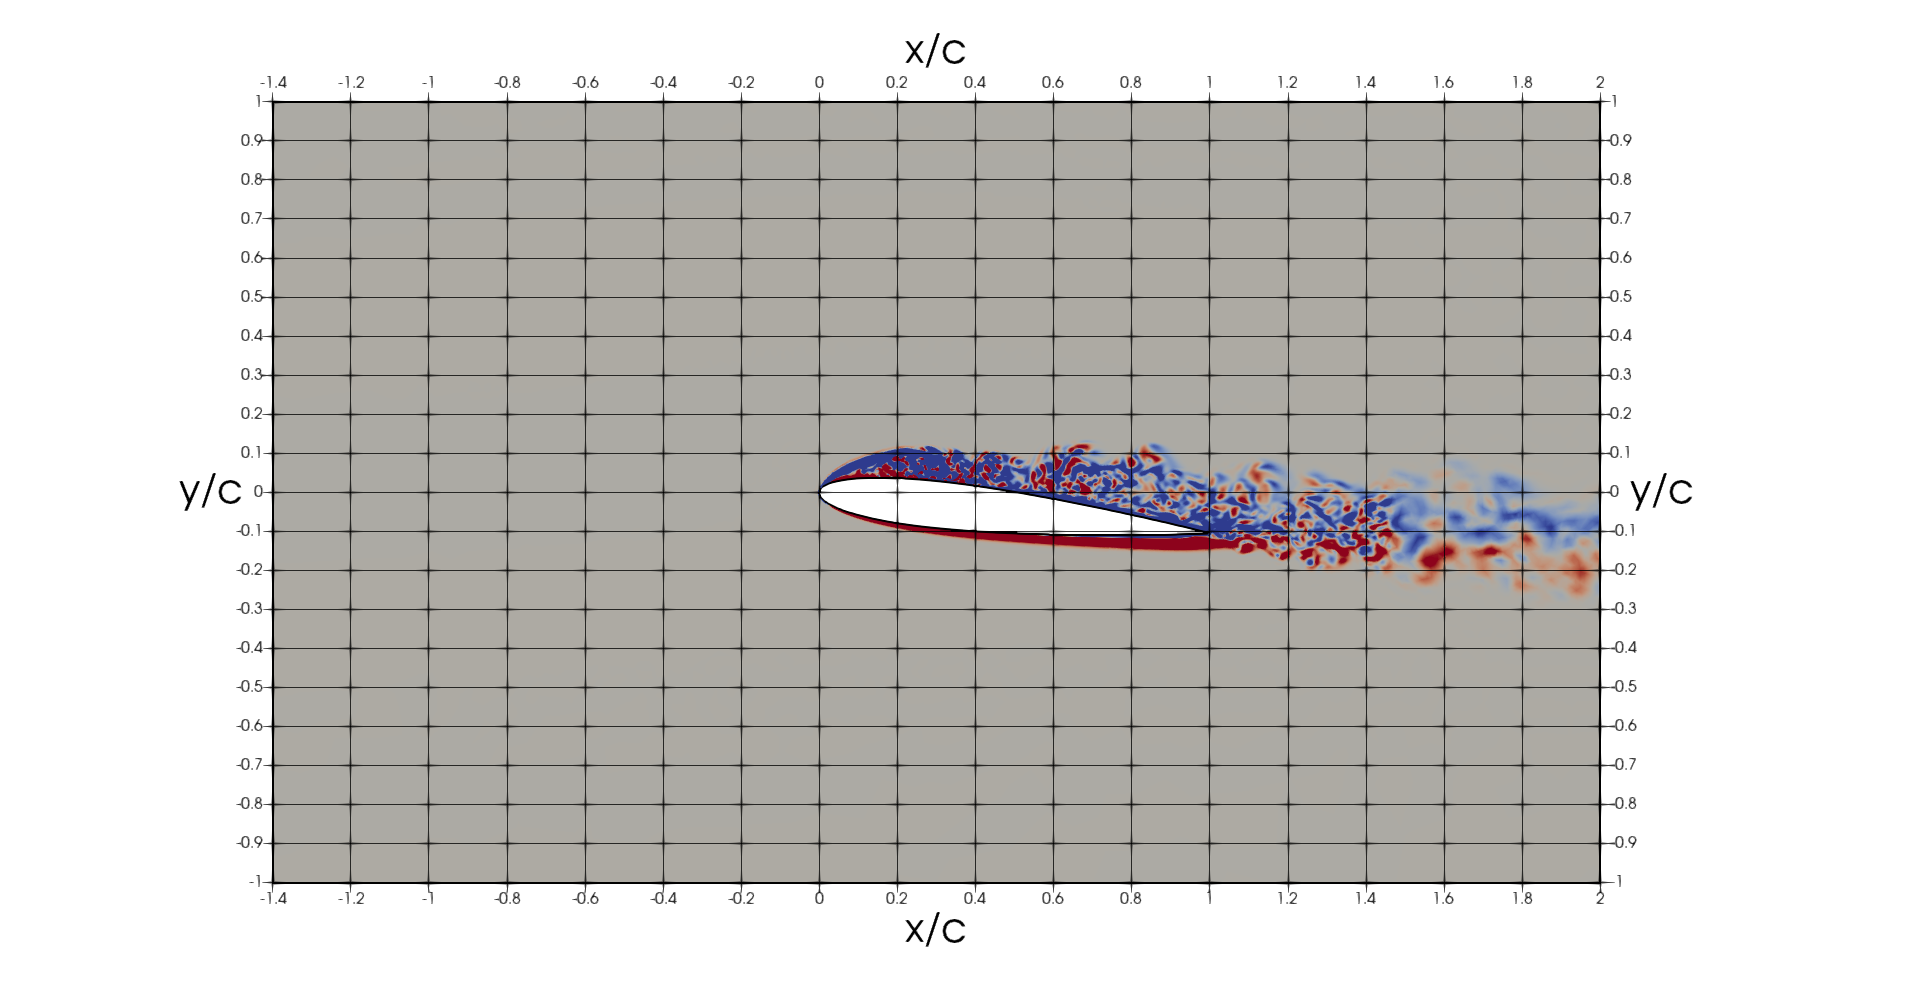
\includegraphics[width=1.25\textwidth]{figures/vorticity_plots/Mza2/ph_210.png}
\caption{Mz\_a2 mesh, $\psi$ = $210^\circ$}
\label{fig:Ma2_psi210}
\end{subfigure}
\begin{subfigure}[b]{0.475\textwidth}
\centering
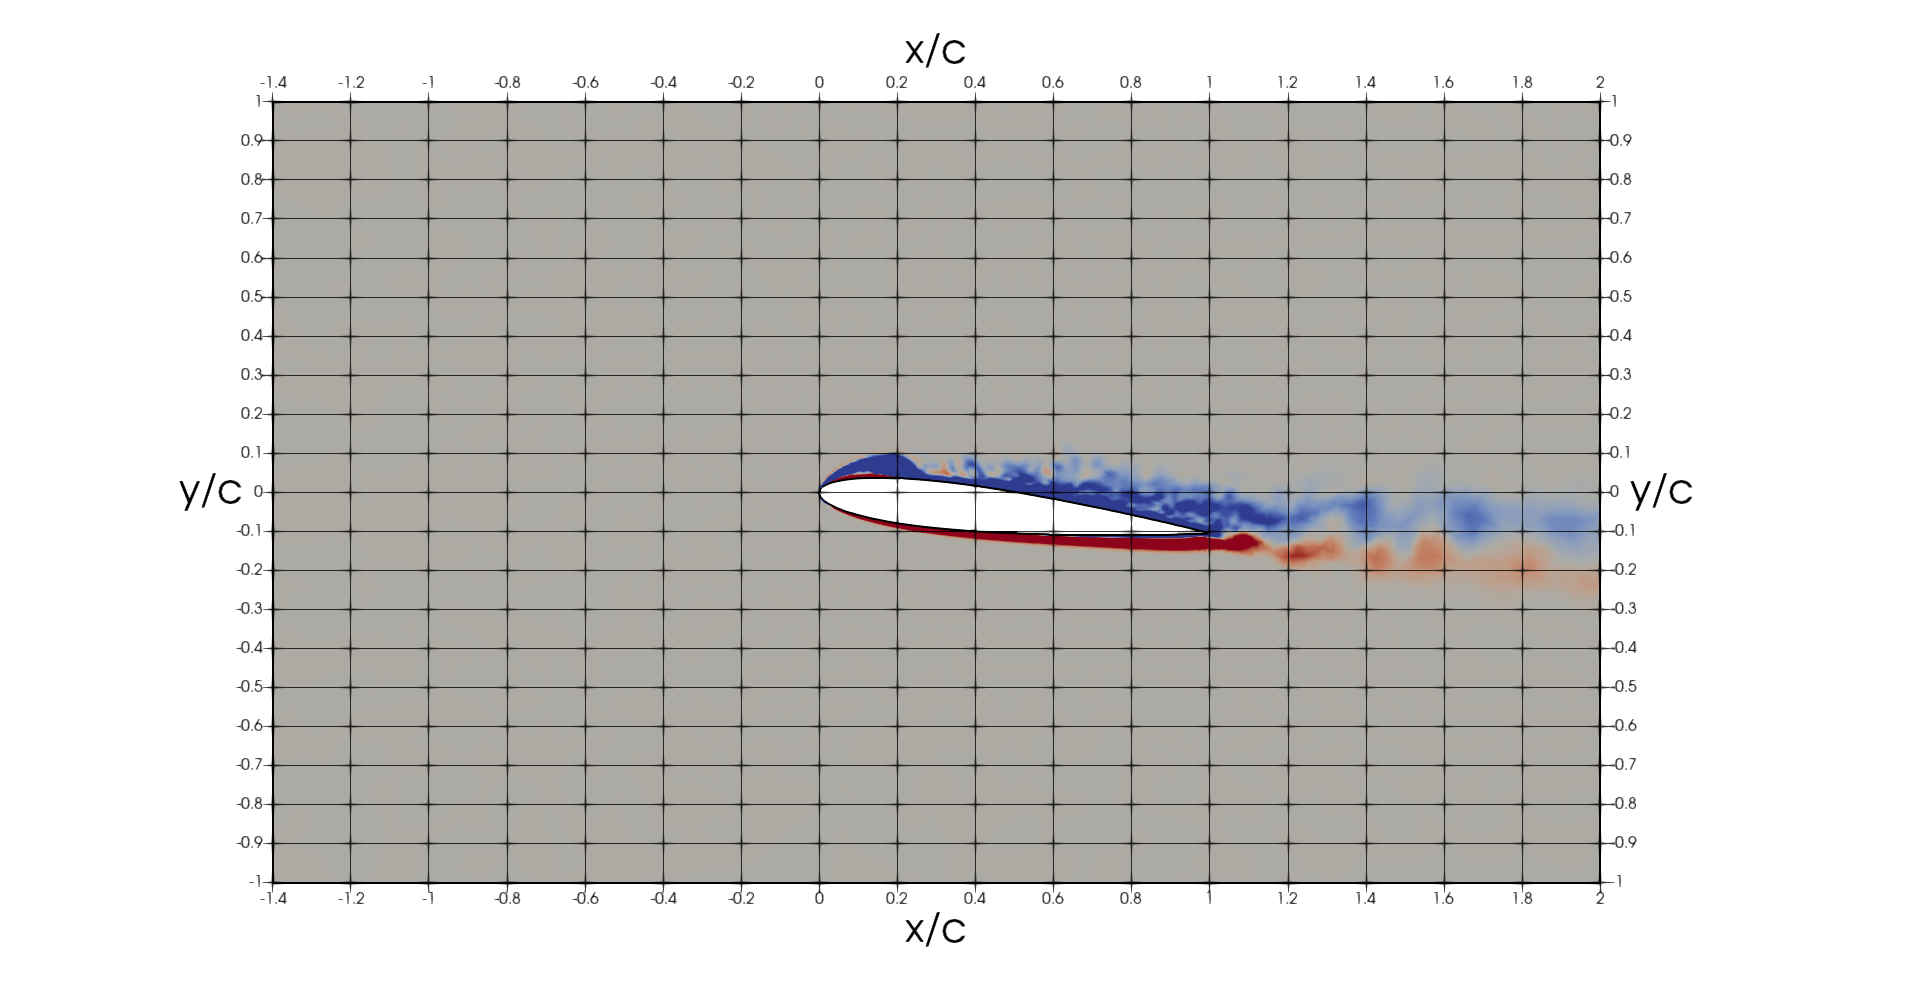
\includegraphics[width=1.25\textwidth]{figures/vorticity_plots/SB/ph_210.png}
\caption{Ms\_a1 mesh, $\psi$ = $210^\circ$}
\label{fig:hadapt_psi210}
\end{subfigure}
\begin{subfigure}[b]{0.475\textwidth}
\centering
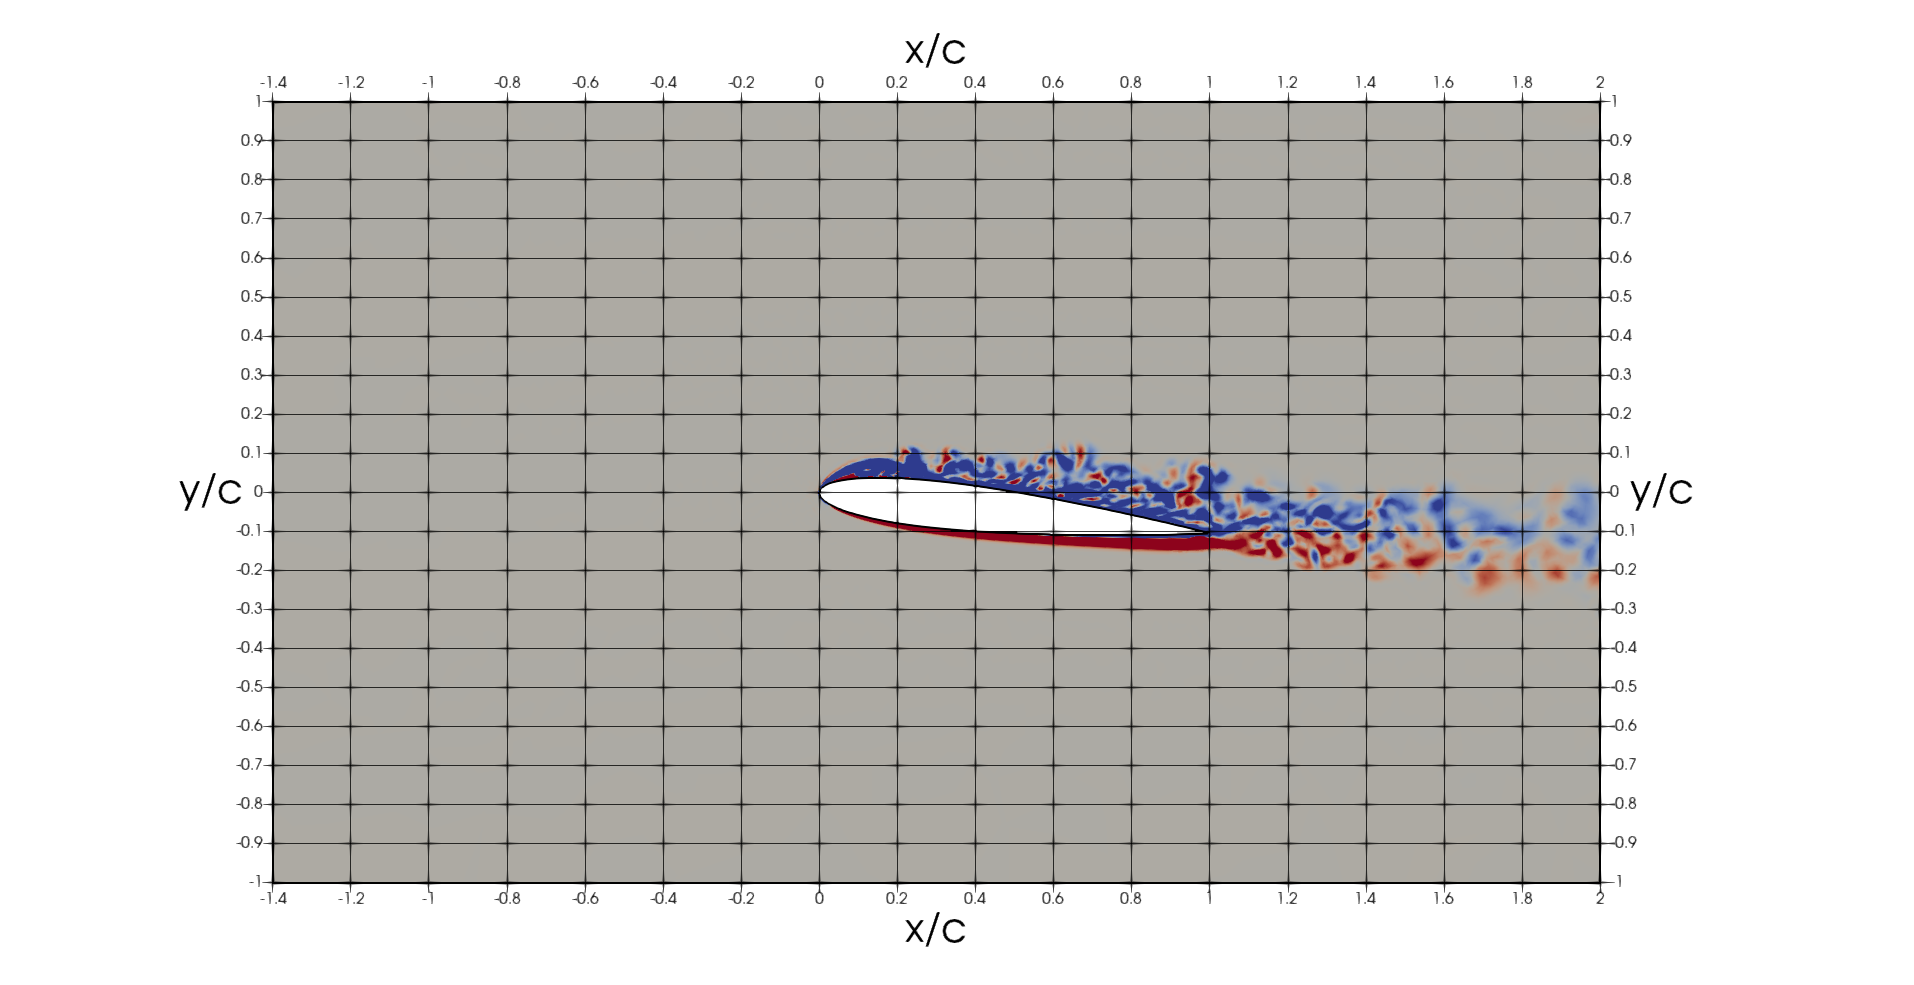
\includegraphics[width=1.25\textwidth]{figures/vorticity_plots/FB/ph_210.png}
\caption{Mf\_a1 mesh, $\psi$ = $210^\circ$}
\label{fig:FB_psi210}
\end{subfigure}
\caption{Spanwise vorticity comparison at $\psi$ = $210^\circ$ for different meshes}
\label{fig:vorticity_210}
\end{figure}



%%VORTICITY PLOT
\begin{figure}[H]
\centering

\begin{subfigure}[b]{0.475\textwidth}
\centering
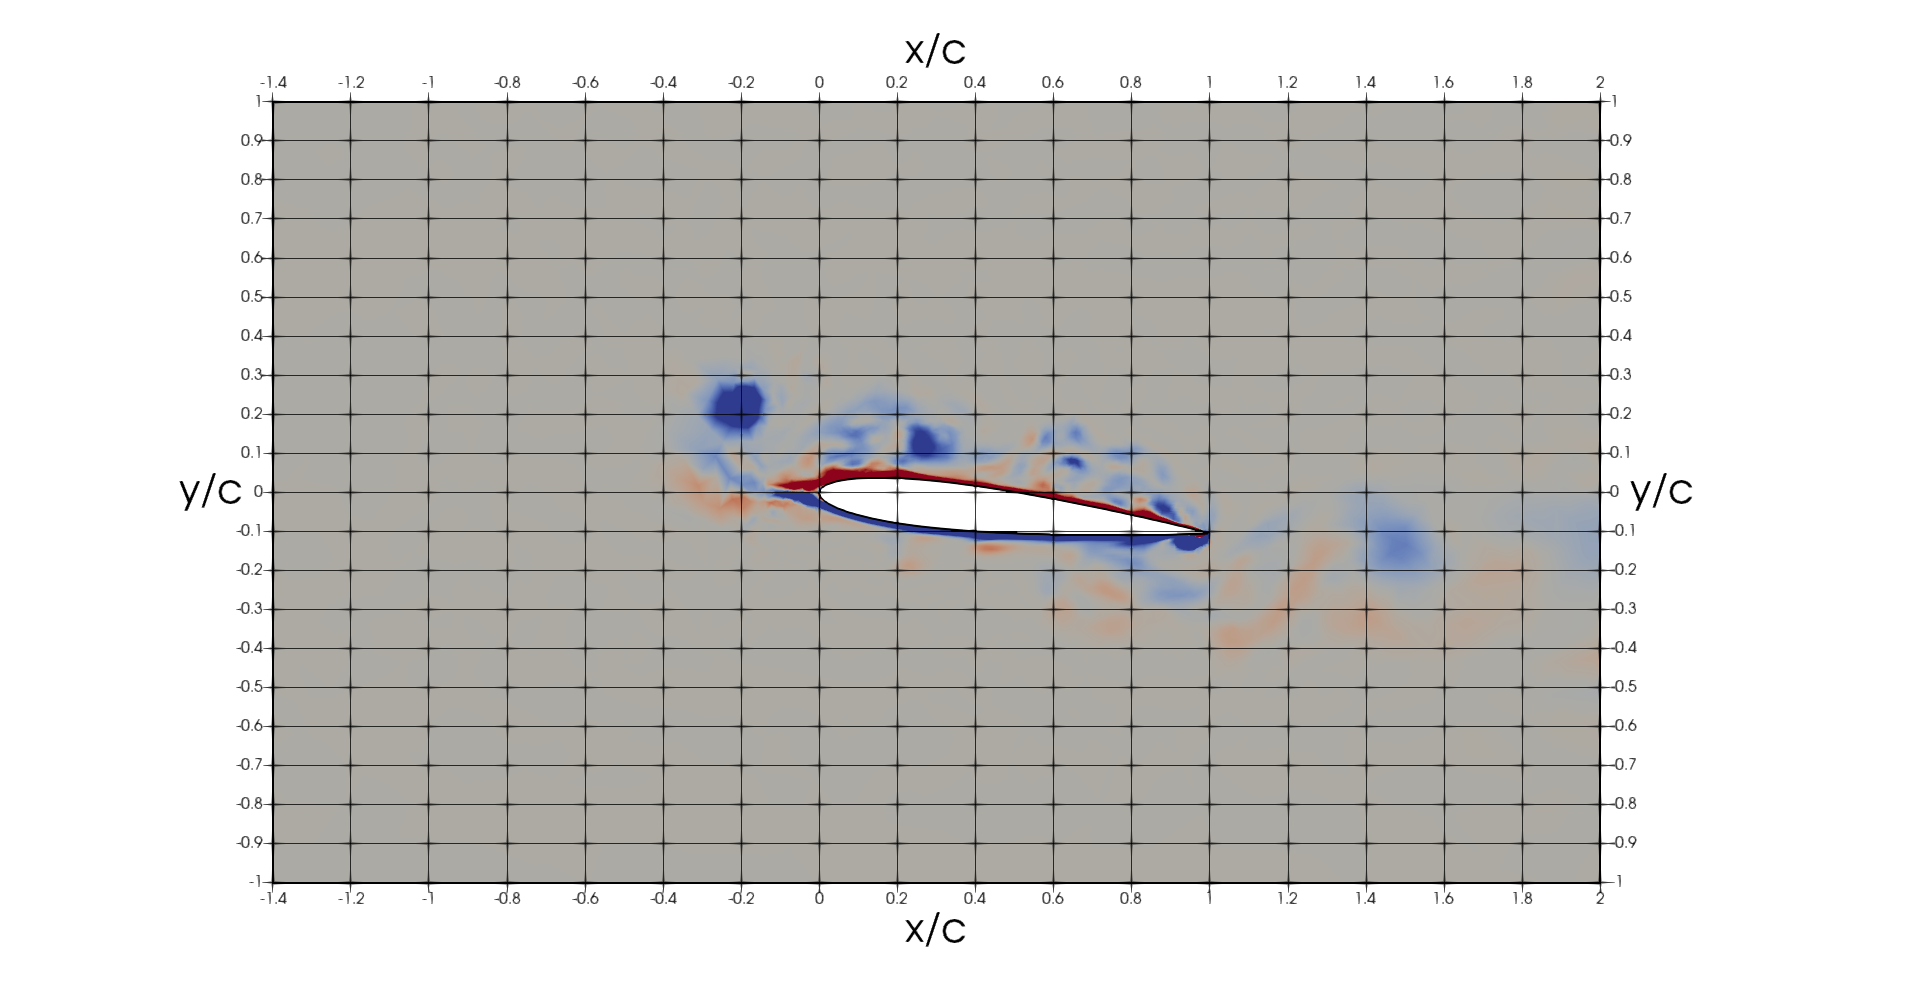
\includegraphics[width=1.25\textwidth]{figures/vorticity_plots/M0/ph_270.png}
\caption{M0 mesh, $\psi$ = $270^\circ$}
\label{fig:M0_psi270}
\end{subfigure}
\begin{subfigure}[b]{0.475\textwidth}
\centering
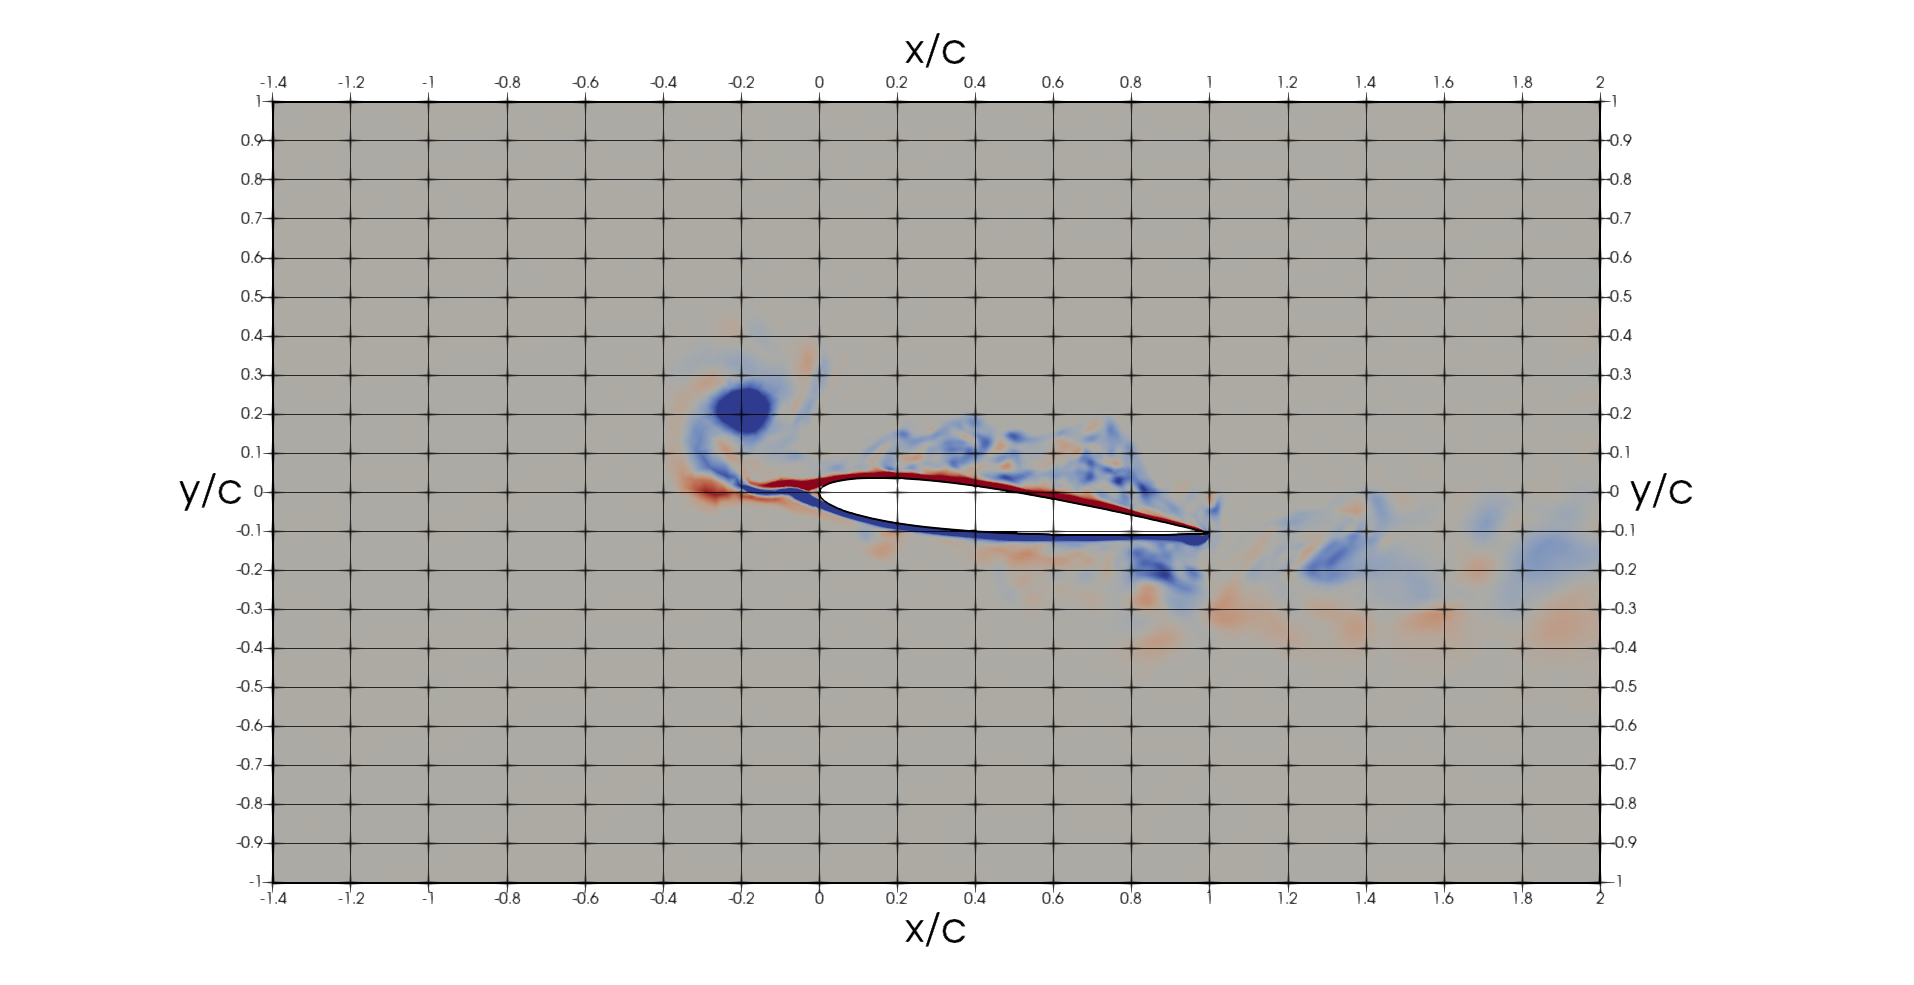
\includegraphics[width=1.25\textwidth]{figures/vorticity_plots/Mza1/ph_270.png}
\caption{Mz\_a1 mesh, $\psi$ = $270^\circ$}
\label{fig:Ma1_psi270}
\end{subfigure}
\begin{subfigure}[b]{0.475\textwidth}
\centering
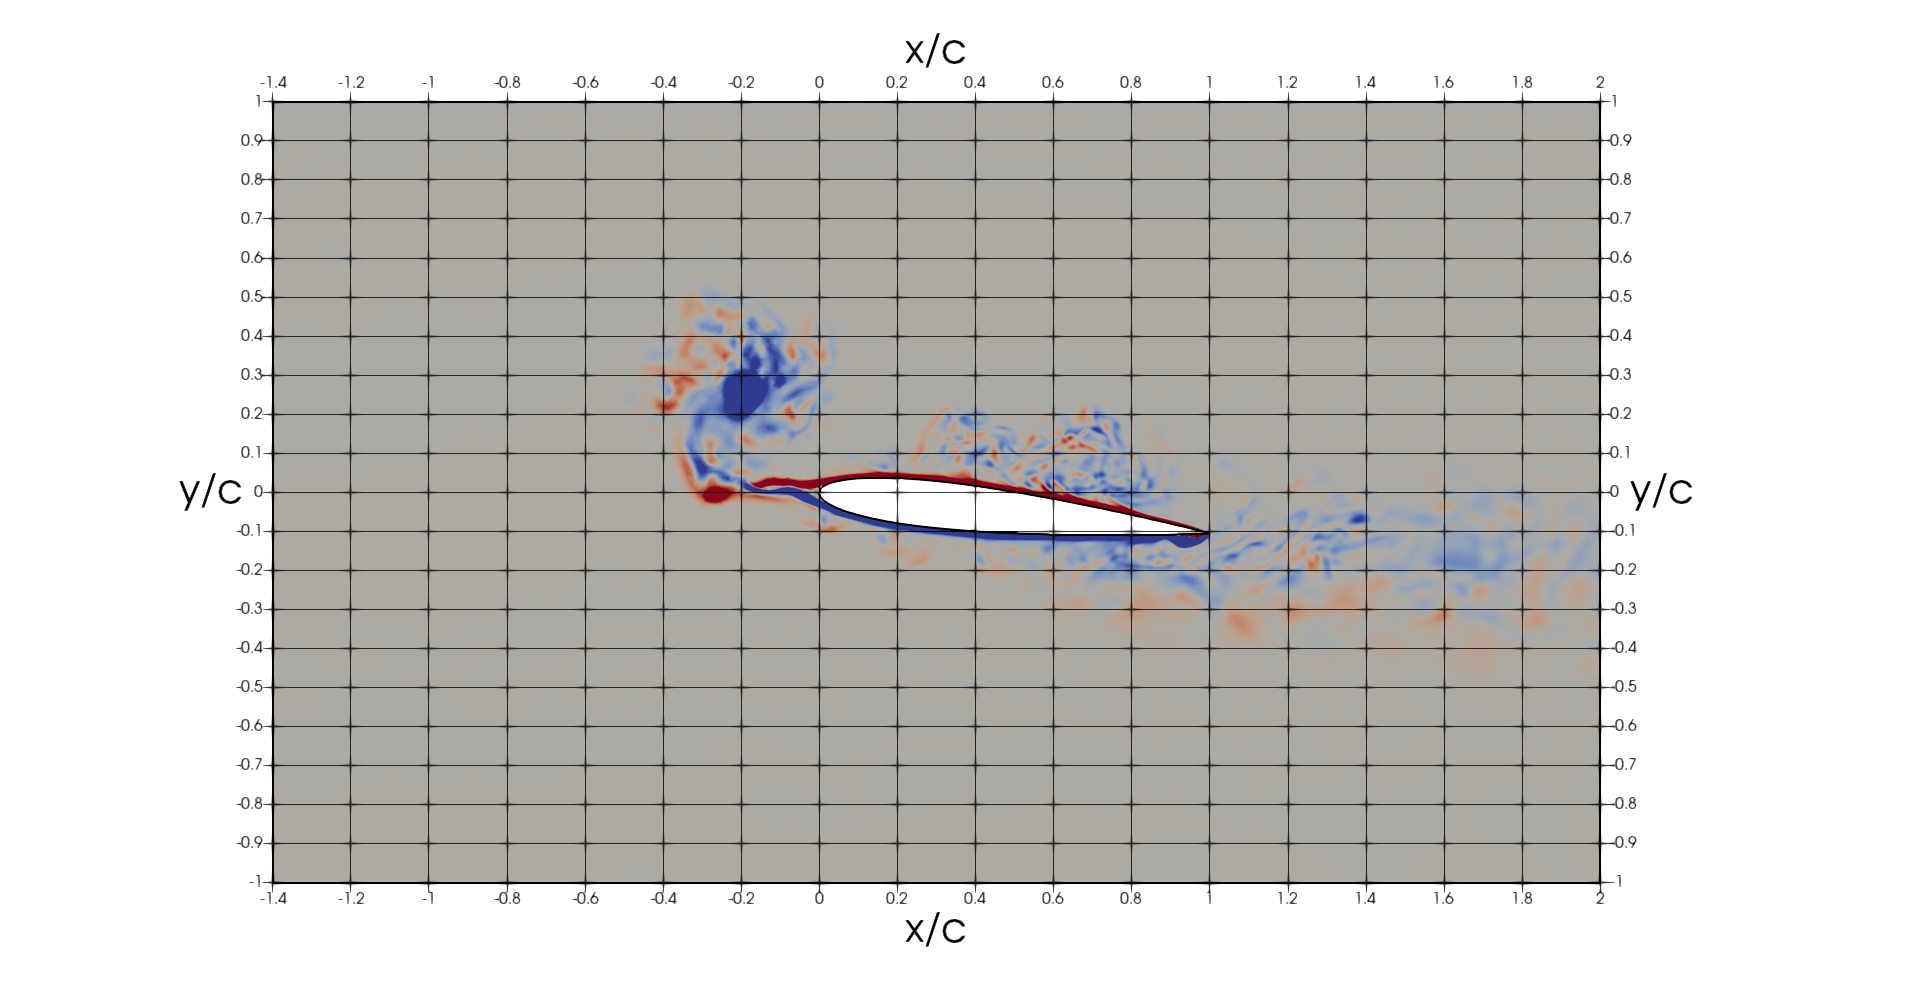
\includegraphics[width=1.25\textwidth]{figures/vorticity_plots/Mza2/ph_270.png}
\caption{Mz\_a2 mesh, $\psi$ = $270^\circ$}
\label{fig:Ma2_psi270}
\end{subfigure}
\begin{subfigure}[b]{0.475\textwidth}
\centering
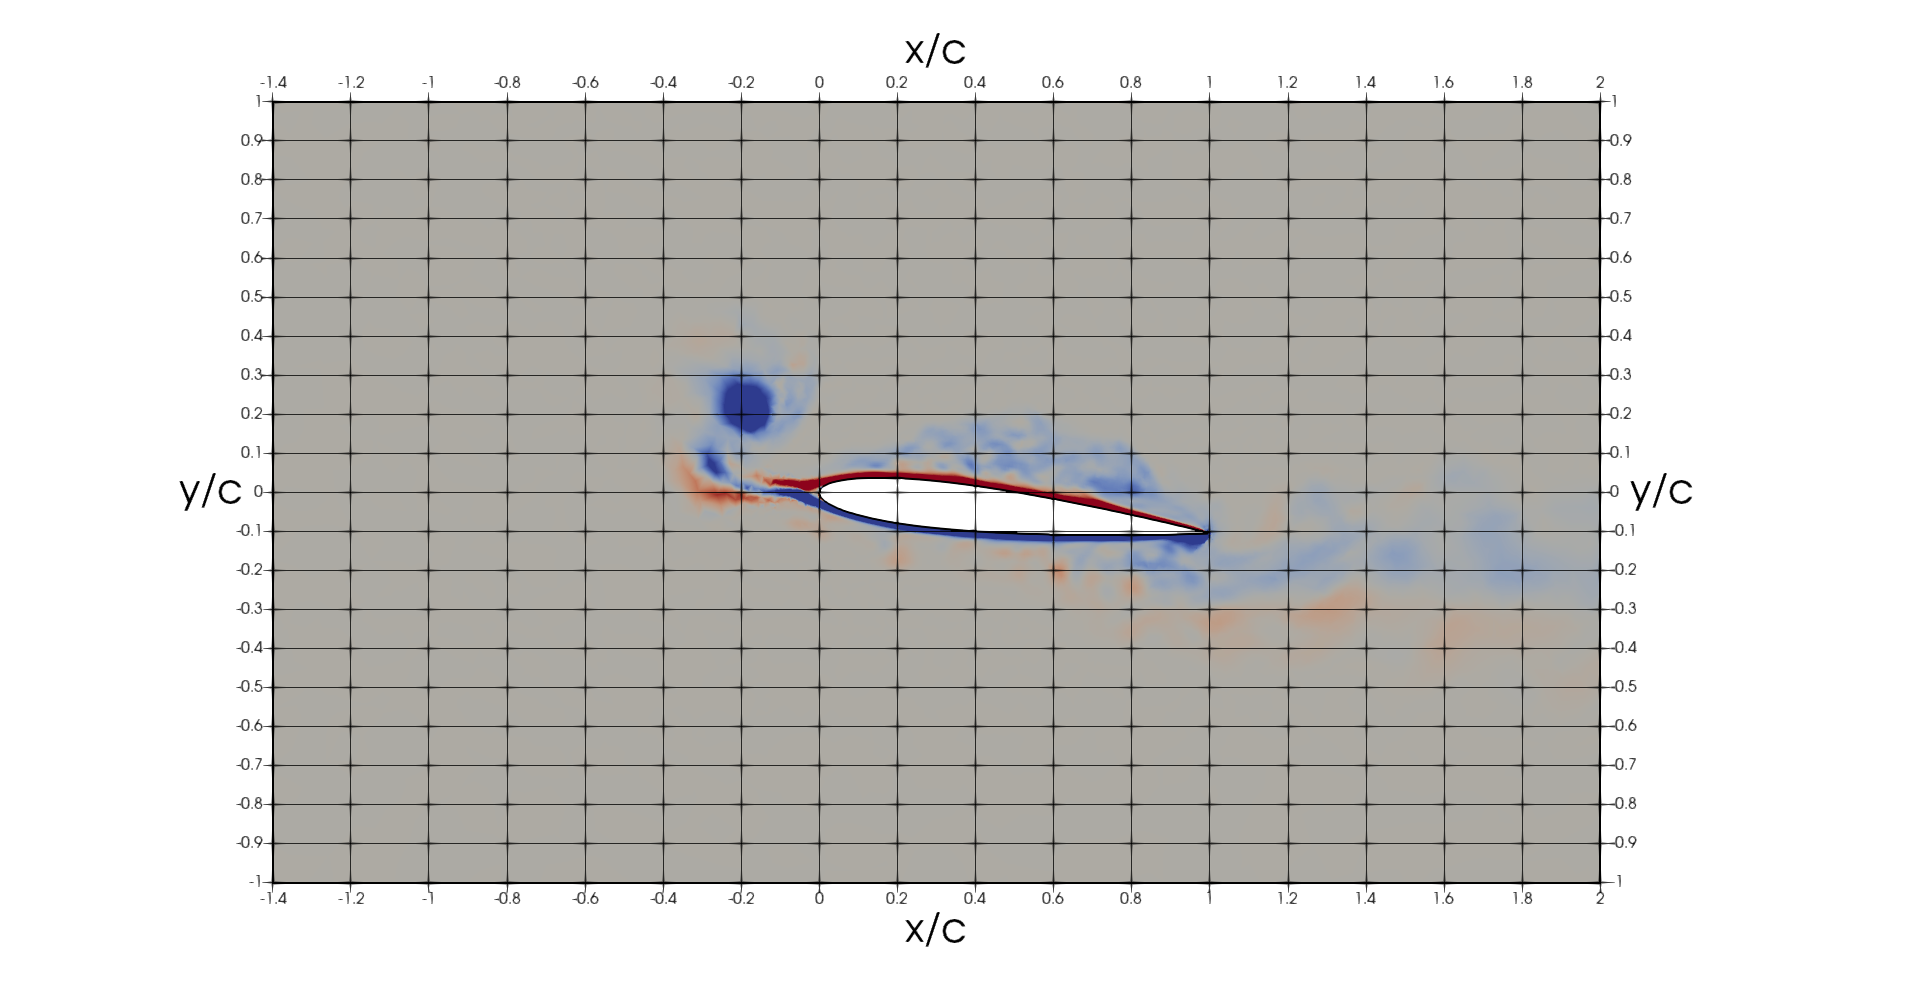
\includegraphics[width=1.25\textwidth]{figures/vorticity_plots/SB/ph_270.png}
\caption{Ms\_a1 mesh, $\psi$ = $270^\circ$}
\label{fig:hadapt_psi270}
\end{subfigure}
\begin{subfigure}[b]{0.475\textwidth}
\centering
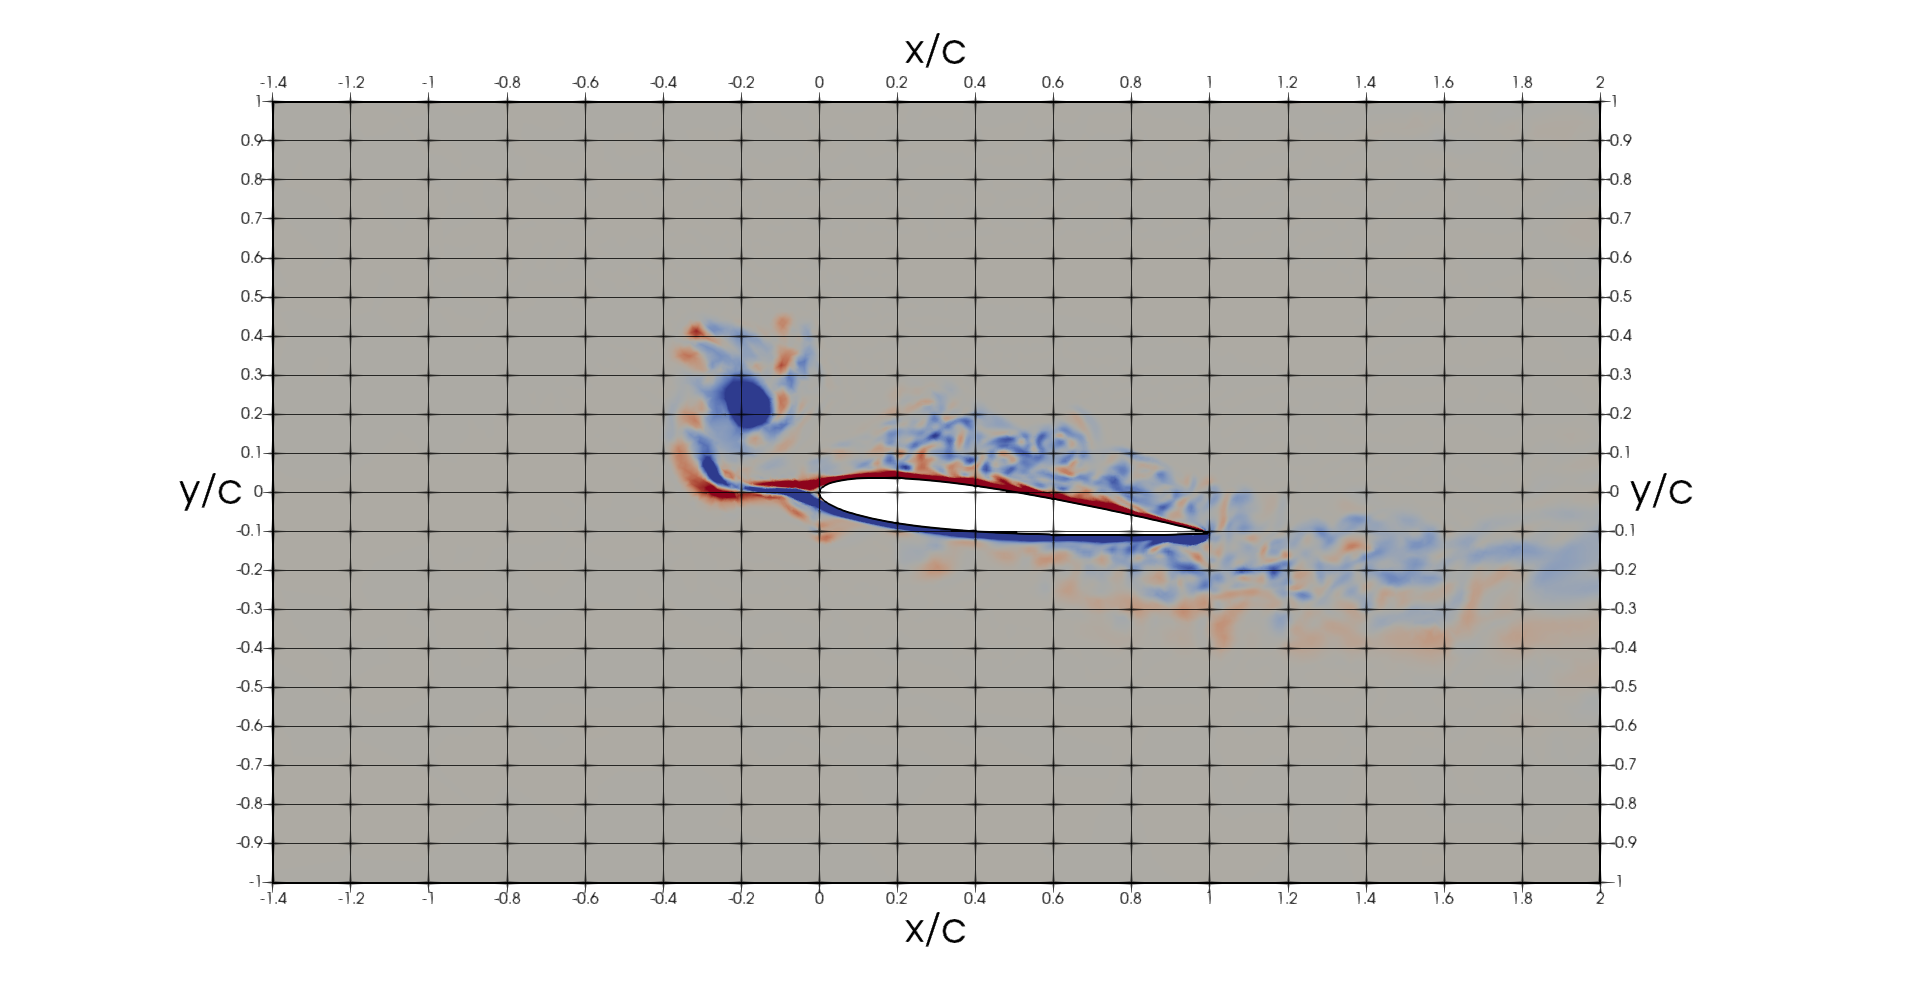
\includegraphics[width=1.25\textwidth]{figures/vorticity_plots/FB/ph_270.png}
\caption{Mf\_a1 mesh, $\psi$ = $270^\circ$}
\label{fig:FB_psi270}
\end{subfigure}
\caption{Spanwise vorticity comparison at $\psi$ = $270^\circ$ for different meshes}
\label{fig:vorticity_270}
\end{figure}

For a more quantitative comparison, we focus on $C_p$  at different phases of interest leading up to LEV formation. $C_p$ is shown in Figure \ref{fig:Cp_plots} at six phases for all meshes. At $\psi=180^\circ$, we can see that flow has started to separate for Mz\_a2 mesh around $x/c=0.1$, whereas for all the other meshes, the flow remains attached. For $\psi=195^\circ$, Mz\_a2 and Ms\_a1 meshes show clear signs of separation and LEV formation/boundary layer roll-up, whereas the other meshes do not. Although note that the location and $C_p$ curve for Mz\_a2 and Ms\_a2 meshes are quite different, and separation is detected further downstream for Mz\_a2. For $\psi=210^\circ$, LEV formation is seen for all meshes 
apart from M0 mesh. $\psi=225^\circ$ shows LEV formation and flow separation for all meshes, with clear differences in separation location and $C_p$ curve for all the meshes. Note that the y-axis limits vary for different phases to highlight differences in $C_p$,.
$\psi=270^\circ$ and $\psi=285^\circ$ also show differences in $C_p$ at the geometric trailing edge when the trailing edge vortex starts forming. 

%%Cp plots

\begin{figure}[H]
\centering

\begin{subfigure}[b]{0.475\textwidth}
\centering
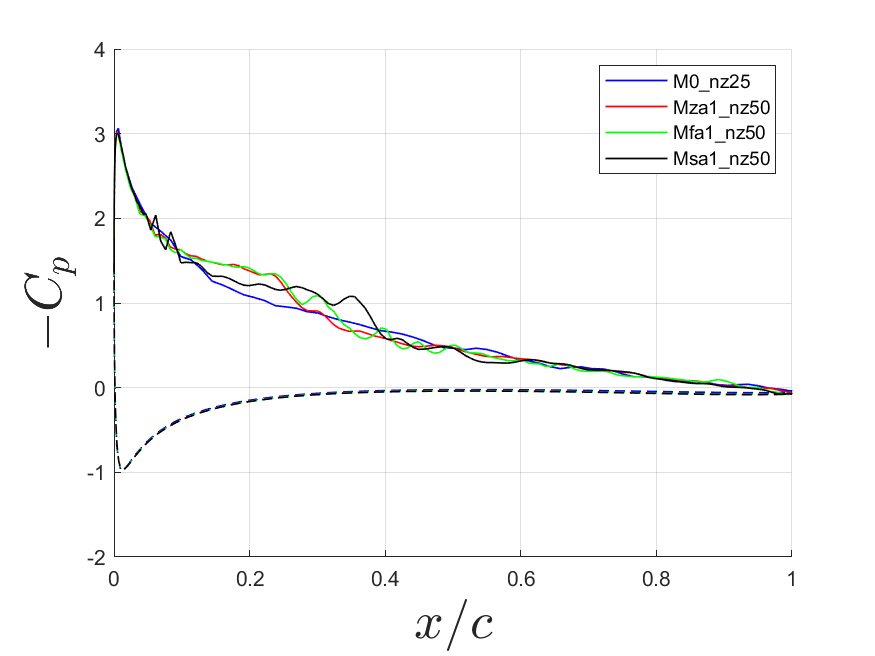
\includegraphics[width=1\textwidth]{figures/Results/Cp_plots/Cp_ph_180.png}
\caption{ $C_p$ at $\psi$ = $180^\circ$}
\label{fig:Cp_180}
\end{subfigure}
\begin{subfigure}[b]{0.475\textwidth}
\centering
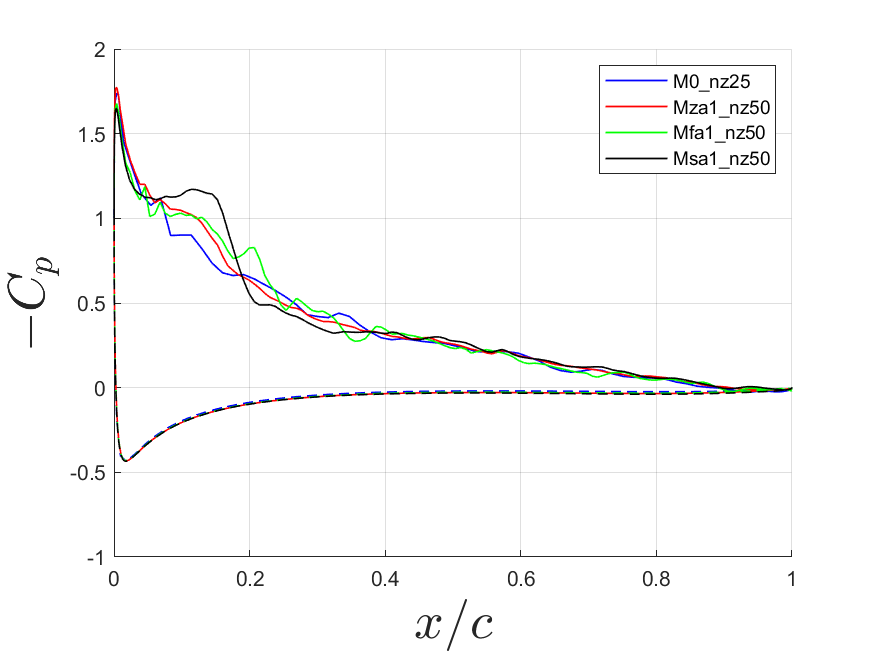
\includegraphics[width=1\textwidth]{figures/Results/Cp_plots/Cp_ph_195.png}
\caption{ $C_p$ at $\psi$ = $195^\circ$}
\label{fig:Cp_195}
\end{subfigure}
\begin{subfigure}[b]{0.475\textwidth}
\centering
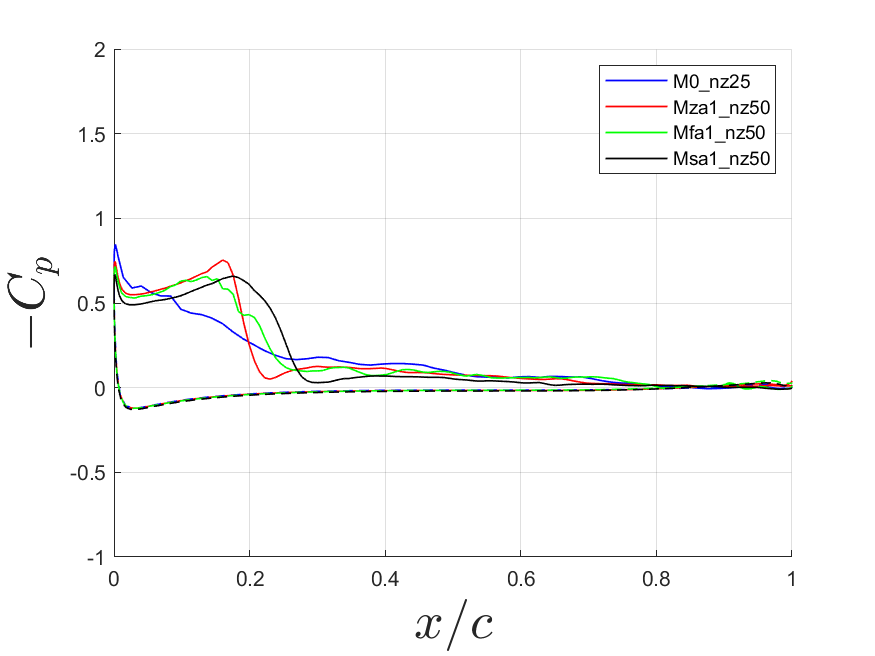
\includegraphics[width=1\textwidth]{figures/Results/Cp_plots/Cp_ph_210.png}
\caption{ $C_p$ at $\psi$ = $210^\circ$}
\label{fig:Cp_210}
\end{subfigure}
\begin{subfigure}[b]{0.475\textwidth}
\centering
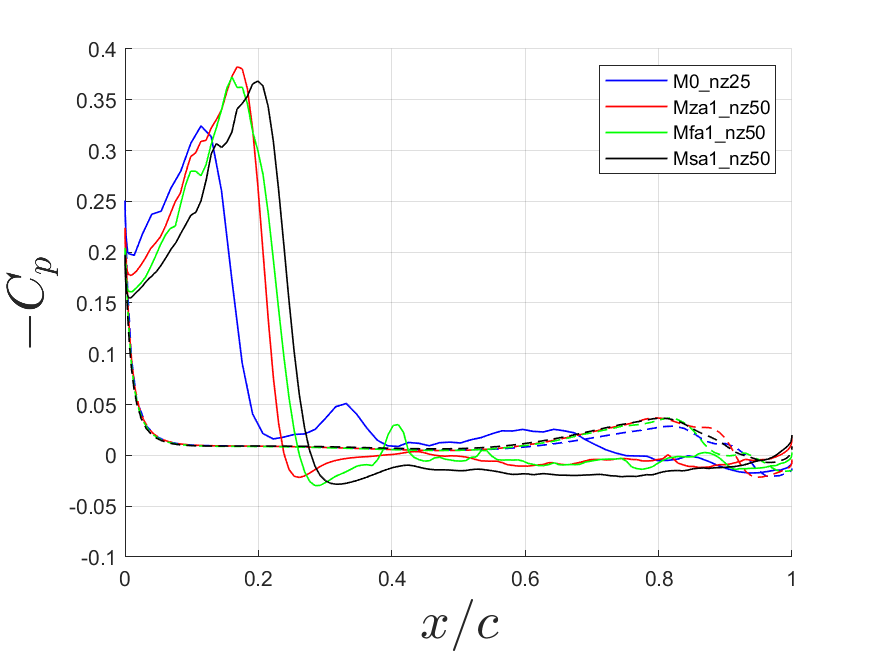
\includegraphics[width=1\textwidth]{figures/Results/Cp_plots/Cp_ph_225.png}
\caption{ $C_p$ at $\psi$ = $225^\circ$}
\label{fig:Cp_225}
\end{subfigure}
\begin{subfigure}[b]{0.475\textwidth}
\centering
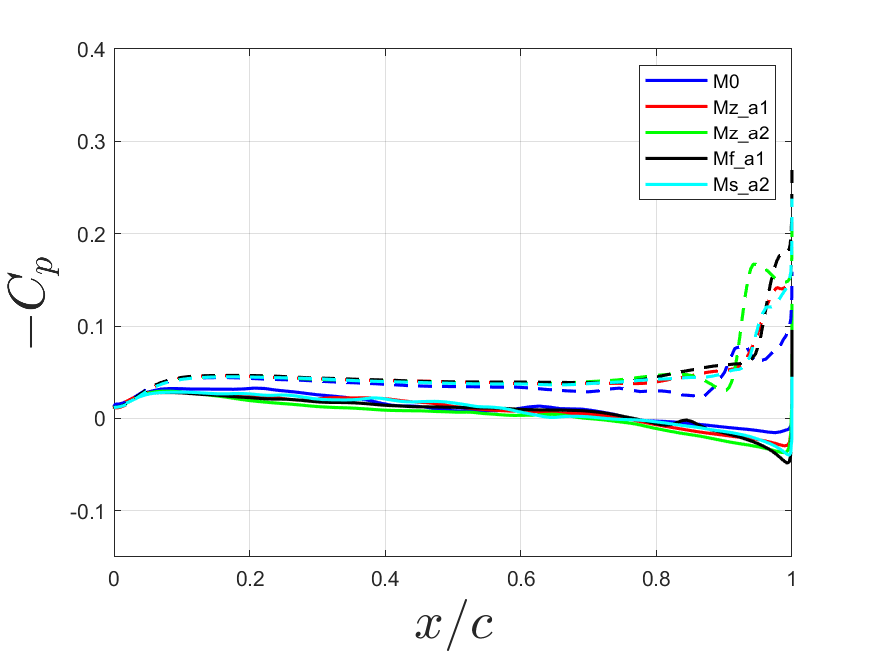
\includegraphics[width=1\textwidth]{figures/Results/Cp_plots/Cp_ph_270.png}
\caption{ $C_p$ at $\psi$ = $270^\circ$}
\label{fig:Cp_270}
\end{subfigure}
\begin{subfigure}[b]{0.475\textwidth}
\centering
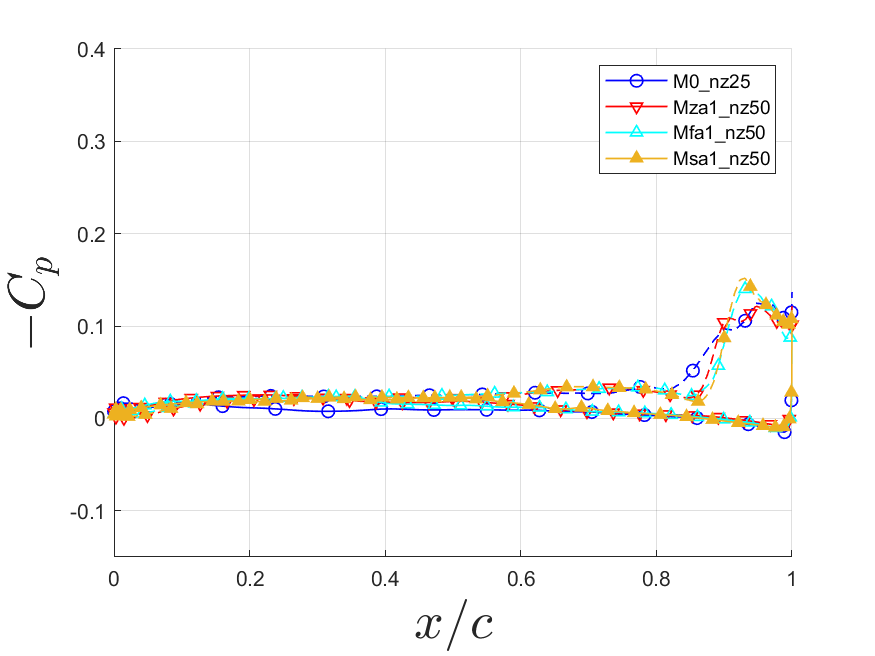
\includegraphics[width=1\textwidth]{figures/Results/Cp_plots/Cp_ph_285.png}
\caption{ $C_p$ at $\psi$ = $285^\circ$}
\label{fig:Cp_285}
\end{subfigure}
\caption{$C_p$ comparison for different meshes. Top surface $C_p$ is denoted by solid lines and bottom surface $C_p$ is denoted by dashed lines}
\label{fig:Cp_plots}
\end{figure}

For the LEV, a quantitative comparison is performed for the circulation which is calculated based on the Lamb-Oseen vortex model. The circulation is shown for all meshes in Figure \ref{fig:circulation} (over the relevant lifetime of LEV). As compared to Mz\_a2, circulation of the LEV is under predicted by all meshes, with M0 having the lowest circulation value through all the phases. Also note that circulation for Mz\_a2 after $\psi=255$ remains fairly constant, whereas for the other meshes, it marginally increases with phase. 

\begin{figure}[H]
\centering
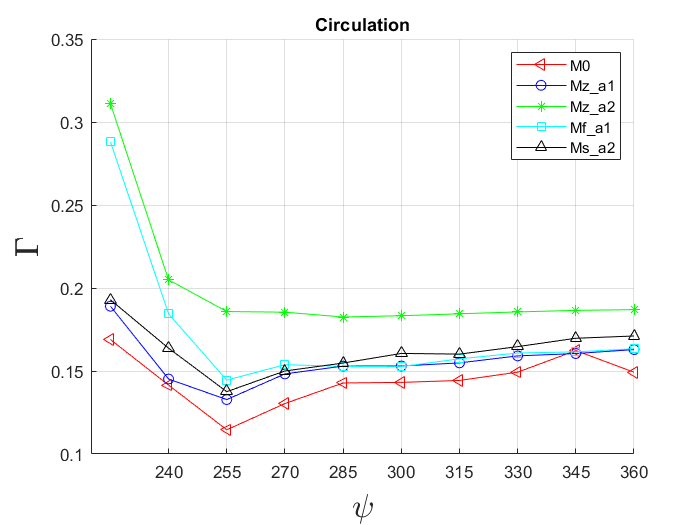
\includegraphics[width=0.7\textwidth]{figures/Results/circulation.png}
\caption{LEV circulation for different meshes}
\label{fig:circulation}
\end{figure}

In summary, mesh refinement/adaptation is necessary to perform accurate LES of complex aerodynamic problems.